% !TeX root = enterprise-architecture-digital-blueprint.tex
% !TeX encoding = UTF-8
\chapter{Gap Analysis dan Paket Kerja}
\label{ch:ch11}

\section*{Tujuan Pembelajaran}
\begin{itemize}
  \item Menyusun \textit{gap analysis} lintas domain dengan membandingkan kondisi saat ini dan kondisi target.
  \item Mengelompokkan gap menjadi paket kerja (\textit{work package}) dengan ruang lingkup yang jelas.
  \item Menganalisis dependensi antarpaket kerja dan dampaknya pada pemangku kepentingan.
\end{itemize}

\section{Pendahuluan}

Misalkan tim arsitektur Medikara selesai memaparkan rancangan target di depan
direksi. Di layar terlihat Sistem Informasi Manajemen Rumah Sakit (SIMRS)
terpadu, Master Patient Index (MPI), platform integrasi, platform data, dan
portal mitra. Semua direktur setuju bahwa gambarnya bagus. Direktur keuangan
lalu bertanya: ``Mana yang dikerjakan lebih dahulu, siapa penanggung jawabnya,
dan dari mana direksi tahu pekerjaan itu selesai?'' Gambar itu tidak memberi
jawaban. Rancangan target yang berhenti di sini hanyalah daftar keinginan yang
rapi. Kotak aplikasi baru tidak menjelaskan cara membersihkan identitas, melatih
petugas, mengubah kontrak, atau menghentikan fungsi lama. Tanpa analisis selisih,
peta jalan berubah menjadi urutan pengadaan yang kehilangan hubungan dengan
masalah organisasi.

Bab ini menjembatani kondisi saat ini pada tonggak C2 dan rancangan target dari
Bab 8 sampai Bab 10. Selisih keduanya dikaji lintas domain, lalu dikelompokkan
menjadi paket kerja yang memiliki hasil, batas, pemilik, dan bukti penerimaan.
Dependensi dan dampaknya diperiksa sebelum tim memberi tanggal. Perbandingan kondisi awal dan target perlu memperlihatkan unsur yang
tetap, baru, sengaja dihapus, serta tidak sengaja terlewat. Hasil bab ini menutup tonggak C3 dan menjadi masukan langsung bagi
arsitektur transisi pada Bab 12.

\IfFileExists{../figures/ch11-diagram-konsep.png}{%
Gambar \ref{fig:ch11-ilustrasi-bab} merangkum hubungan komponen dan konsep utama bab ini.
\begin{figure}[!htb]
  \centering
  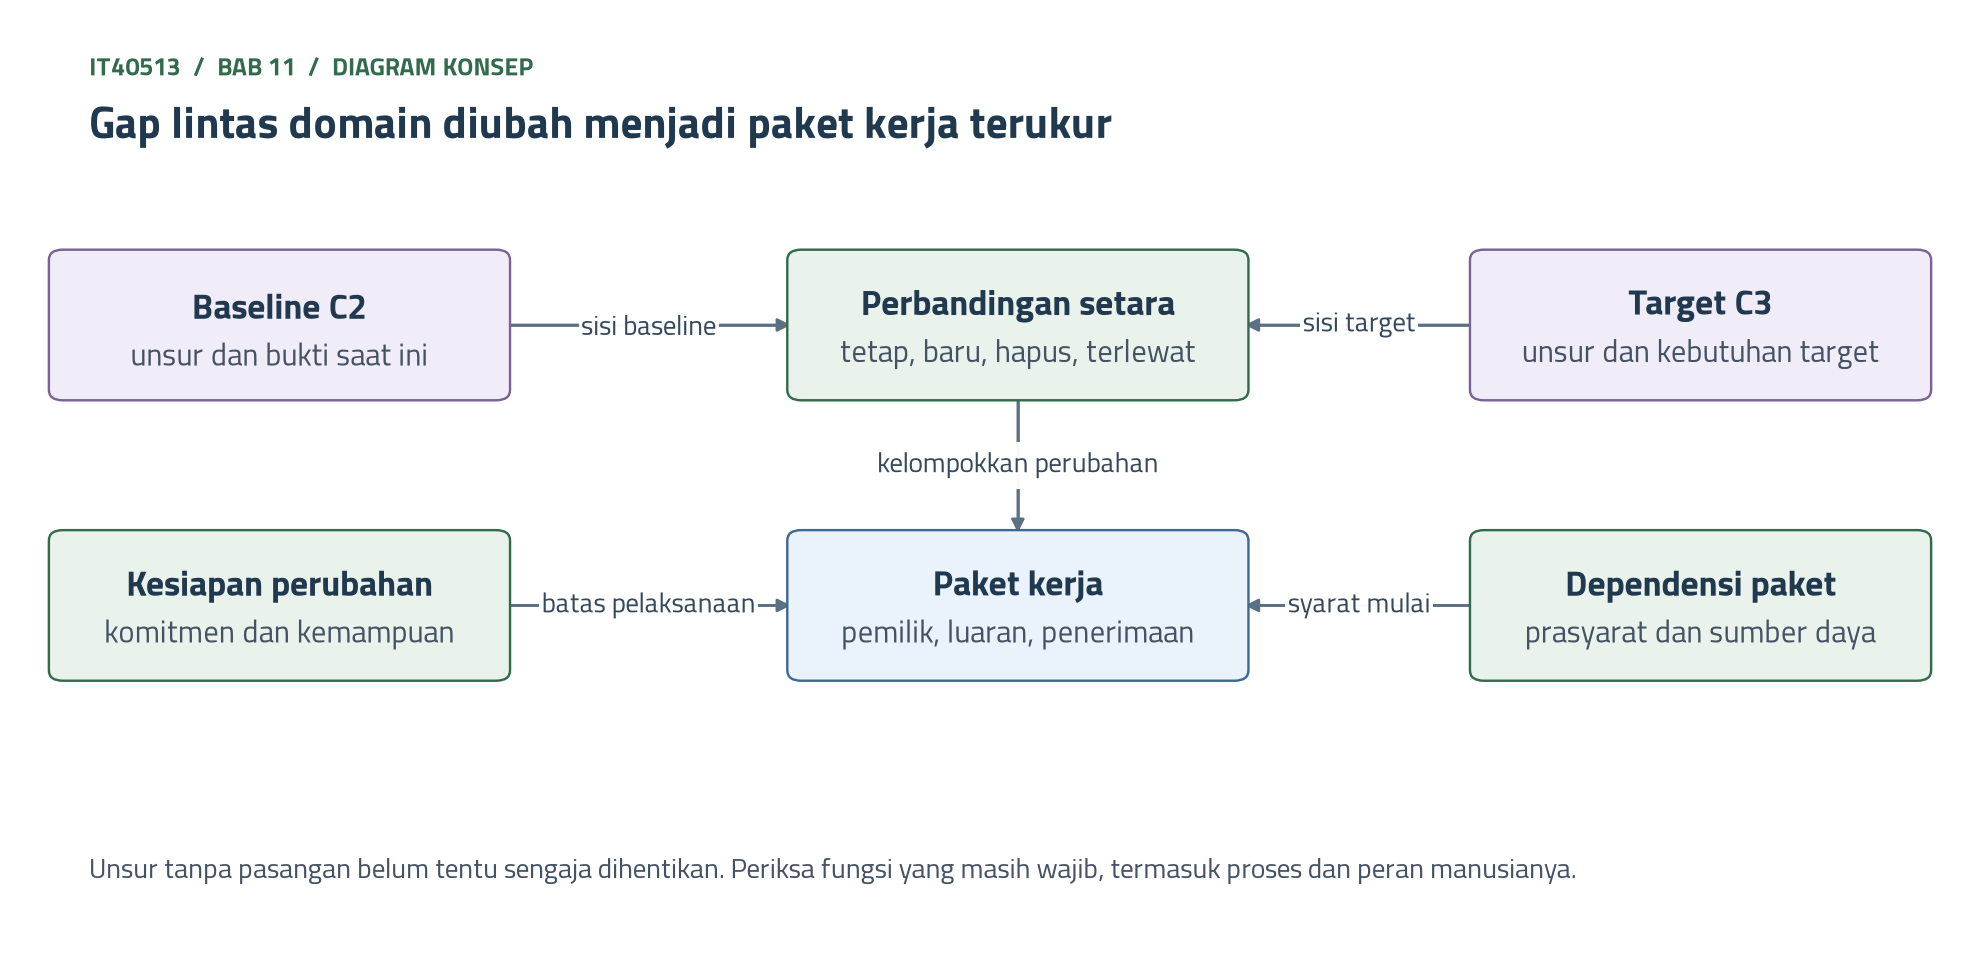
\includegraphics[width=\textwidth]{../figures/ch11-diagram-konsep.png}
  \caption{Gap lintas domain diubah menjadi paket kerja terukur}
  \label{fig:ch11-ilustrasi-bab}
\end{figure}
}{}

Rujukan utama bab ini adalah The Open Group Architecture Framework (TOGAF). Teknik
\textit{gap analysis} termasuk bagian ADM Techniques pada TOGAF 10 \cite{togaf10}.
Rumusan yang dipakai di sini dicocokkan dengan bab Gap Analysis pada TOGAF 9
\cite{c11-togaf9-gap}. Konsolidasi gap menjadi paket kerja berada pada fase E
Architecture Development Method (ADM) \cite{c11-togaf-fasee}, dan elemen
implementasi serta migrasi mengikuti ArchiMate 3.2 \cite{archimate32}. Jenis
dependensi mengikuti Malone dan Crowston \cite{c11-malone1994}. Matriks dependensi
berasal dari Steward serta Browning \cite{c11-steward1981,c11-browning2001}.
Kesiapan perubahan mengikuti Weiner serta Armenakis dan rekan
\cite{c11-weiner2009,c11-armenakis1993}. Model dan matriks membantu menelusuri
alasan perubahan, tetapi keduanya tidak menggantikan keputusan pemilik layanan.

\section{Teknik Gap Analysis dalam TOGAF}

\textit{Gap analysis} membandingkan arsitektur awal (\textit{baseline}) dengan
arsitektur target pada lingkup yang sama. TOGAF memakai teknik ini untuk
memvalidasi arsitektur yang sedang disusun. Gagasan dasarnya adalah memperlihatkan
selisih keduanya, yaitu unsur yang sengaja dihilangkan, unsur yang tidak sengaja
terlewat, dan unsur yang belum didefinisikan \cite{c11-togaf9-gap}. Alatnya berupa
matriks. Seluruh blok bangun arsitektur (\textit{architecture building block})
kondisi awal ditulis pada sumbu tegak, dan seluruh blok kondisi target pada sumbu
datar. Satu baris \textit{New} dan satu kolom \textit{Eliminated} ditambahkan di
ujung matriks.

Cara membaca selnya sederhana. Unsur yang ada di kedua sisi ditandai
\textit{Included}. Unsur awal yang tidak ada di target ditandai \textit{Eliminated}
bila memang sengaja dihentikan. Bila ternyata terlewat, unsur itu dikembalikan pada
iterasi rancangan berikutnya. Unsur target yang tidak ada di kondisi awal ditandai
pada baris \textit{New} sebagai gap yang ditutup dengan membangun atau membeli
\cite{c11-togaf9-gap}.

Perbandingan memerlukan padanan kode atau aturan pemetaan. Mengganti nama ``SIMRS
Bekasi'' menjadi ``Layanan Klinis Terpadu'' tidak membuktikan bahwa semua fungsi
lama sudah ditangani. Fungsi pelaporan, arsip, dan pengecualian operasional perlu
ditelusuri satu per satu. Tim membandingkan kemampuan serta hubungan, bukan hanya
nama kotak.

Analoginya seperti pindah rumah. Daftar isi rumah lama dan denah rumah baru membantu
menentukan barang yang dibawa, diperbaiki, dibeli, atau dilepas. Lemari yang tidak
muncul pada denah baru perlu keputusan: isinya dipindahkan ke mana? Menganggap
barang yang tidak digambar pasti tidak dibutuhkan dapat menghilangkan dokumen
penting.

Dua contoh dari Medikara Health:
\begin{enumerate}
  \item Bab 9 mencatat 2,1 juta catatan identitas di tujuh sumber, untuk sekitar
        1,5 juta orang. Target menghubungkan semuanya lewat MPI, tetapi nomor rekam
        medis lokal tetap tercetak di label sampel, gelang pasien, dan arsip kertas.
        Gap tidak ditulis ``hapus semua nomor lama'', melainkan kemampuan memetakan,
        menelusuri asal, dan mengoreksi salah cocok.
  \item ERP (\textit{Enterprise Resource Planning}) keuangan ada di kedua sisi,
        sehingga ditandai tetap. Tanda itu tidak berarti tanpa pekerjaan. Bab 9
        menambahkan antarmuka tagihan dan klaim, karena klaim Badan Penyelenggara
        Jaminan Sosial (BPJS) yang dikembalikan harus turun dari 9 persen menjadi 3
        persen. Unsur yang dipertahankan tetap dapat menimbulkan perubahan kapasitas,
        konfigurasi, atau kontrak.
\end{enumerate}

Gambar \ref{fig:ch11-matriks-gap} memperlihatkan potongan matriks untuk aplikasi dan
teknologi Medikara. Kata ``Diganti'' dan ``Digabung'' adalah kesepakatan modul ini
untuk elemen lama yang punya padanan baru, bukan istilah TOGAF.

\begin{figure}[!htb]
  \centering
  \begin{tikzpicture}[
  font=\scriptsize,
  kepala/.style={align=center, font=\tiny\bfseries},
  label/.style={anchor=west, align=left, font=\scriptsize},
  isi/.style={align=center, font=\tiny\bfseries}
]
  % Ukuran: kolom label 3,3 cm, delapan kolom masing-masing 1,08 cm,
  % baris judul 0,9 cm, sembilan baris isi masing-masing 0,66 cm.
  \fill[praditagreen!15] (0,0) rectangle (11.94,-0.9);

  % Sel berisi, diwarnai sebelum garis kisi digambar.
  \fill[green!10]  (3.30,-0.90) rectangle (4.38,-1.56);
  \fill[blue!8]    (4.38,-1.56) rectangle (5.46,-2.22);
  \fill[blue!8]    (4.38,-2.22) rectangle (5.46,-2.88);
  \fill[blue!8]    (5.46,-2.88) rectangle (6.54,-3.54);
  \fill[blue!8]    (6.54,-3.54) rectangle (7.62,-4.20);
  \fill[blue!8]    (7.62,-4.20) rectangle (8.70,-4.86);
  \fill[gray!35]   (10.86,-4.86) rectangle (11.94,-5.52);
  \fill[red!22]    (10.86,-5.52) rectangle (11.94,-6.18);
  \fill[orange!12] (8.70,-6.18) rectangle (9.78,-6.84);
  \fill[orange!12] (9.78,-6.18) rectangle (10.86,-6.84);

  % Garis kisi.
  \foreach \y in {0,-0.9,-1.56,-2.22,-2.88,-3.54,-4.20,-4.86,-5.52,-6.18,-6.84}
    \draw[gray!60] (0,\y) -- (11.94,\y);
  \foreach \x in {0,3.30,4.38,5.46,6.54,7.62,8.70,9.78,10.86,11.94}
    \draw[gray!60] (\x,0) -- (\x,-6.84);
  \draw[thick] (10.86,0) -- (10.86,-6.84);
  \draw[thick] (0,-6.18) -- (11.94,-6.18);

  % Judul kolom: elemen target, ditambah kolom Dihapus.
  \node[kepala] at (1.65,-0.45) {Baris: \textit{baseline}\\Kolom: target};
  \node[kepala] at (3.84,-0.45) {ERP\\keuangan};
  \node[kepala] at (4.92,-0.45) {SIMRS\\terpadu};
  \node[kepala] at (6.00,-0.45) {Platform\\integrasi};
  \node[kepala] at (7.08,-0.45) {Platform\\data};
  \node[kepala] at (8.16,-0.45) {\textit{Landing}\\\textit{zone}};
  \node[kepala] at (9.24,-0.45) {MPI};
  \node[kepala] at (10.32,-0.45) {Akses\\terpusat};
  \node[kepala] at (11.40,-0.45) {Dihapus};

  % Judul baris: elemen baseline, ditambah baris Baru.
  \node[label] at (0.08,-1.23) {ERP keuangan};
  \node[label] at (0.08,-1.89) {Lima SIMRS lokal};
  \node[label] at (0.08,-2.55) {SIM Klinik};
  \node[label] at (0.08,-3.21) {Integrasi \textit{point-to-point}};
  \node[label] at (0.08,-3.87) {23 laporan \textit{spreadsheet}};
  \node[label] at (0.08,-4.53) {Server lokal rumah sakit};
  \node[label] at (0.08,-5.19) {Antrean Bandung};
  \node[label] at (0.08,-5.85) {Surveilans infeksi Bogor};
  \node[label, font=\scriptsize\bfseries] at (0.08,-6.51) {Baru};

  % Isi sel.
  \node[isi] at (3.84,-1.23) {Tetap};
  \node[isi] at (4.92,-1.89) {Diganti};
  \node[isi] at (4.92,-2.55) {Digabung};
  \node[isi] at (6.00,-3.21) {Diganti};
  \node[isi] at (7.08,-3.87) {Diganti};
  \node[isi] at (8.16,-4.53) {Diganti};
  \node[isi] at (11.40,-5.19) {Sengaja};
  \node[isi] at (11.40,-5.85) {Tidak\\[-2pt]sengaja};
  \node[isi] at (9.24,-6.51) {Baru};
  \node[isi] at (10.32,-6.51) {Baru};

  % Keterangan.
  \node[font=\tiny, text width=11.8cm, align=center] at (5.97,-7.27)
    {Tetap: ada di kedua sisi. Diganti atau digabung: elemen lama punya padanan
     baru. Baru: dibangun, dibeli, atau berlangganan. Dihapus: diperiksa, sengaja
     atau tidak.};
\end{tikzpicture}

  \caption{Potongan matriks gap aplikasi dan teknologi Medikara, dengan baris
           \textit{baseline} dan kolom target}
  \label{fig:ch11-matriks-gap}
\end{figure}

Dari delapan baris kondisi awal, satu baris tetap, lima baris diganti atau digabung,
dan dua baris hilang dari target. Dua elemen target sama sekali baru. Tabel
\ref{tab:ch11-baca-matriks} merangkum arti setiap hasil beserta tindakannya.

\begin{table}[!htb]
  \centering
  \caption{Hasil perbandingan pada matriks gap dan tindakan lanjutnya}
  \label{tab:ch11-baca-matriks}
  \small
  \begin{tabularx}{\textwidth}{>{\raggedright\arraybackslash}p{3.1cm}>{\raggedright\arraybackslash}p{2.0cm}>{\raggedright\arraybackslash}X>{\raggedright\arraybackslash}X}
    \hline
    \textbf{Hasil perbandingan} & \textbf{Istilah TOGAF} & \textbf{Makna} & \textbf{Tindakan} \\ \hline
    Ada di kedua sisi & \textit{Included} & Dipertahankan, mungkin dengan perubahan &
      Periksa atribut, hubungan, kapasitas, dan kontrak \\ \hline
    Hanya di target & \textit{New} & Kemampuan atau komponen baru &
      Tentukan pekerjaan dan penerimaan, lalu bangun atau beli \\ \hline
    Hanya di kondisi awal, sengaja & \textit{Eliminated} & Penghentian yang disetujui &
      Putuskan migrasi fungsi, data, dan arsip \\ \hline
    Hanya di kondisi awal, terlewat & Gap & Kelalaian pada rancangan target &
      Kembalikan pada iterasi rancangan berikutnya \\ \hline
  \end{tabularx}
\end{table}

Tim mencatat alasan di setiap hasil perbandingan. ``Tidak dipakai'' memerlukan bukti
penggunaan dan pemeriksaan kewajiban. ``Harus baru'' memerlukan hubungan ke kebutuhan
atau prinsip. Sel yang kosong bukan otomatis kesalahan, tetapi maknanya perlu
dijelaskan.

\subsection*{Satu matriks atau beberapa?}

Pertanyaan kemudian muncul: berapa matriks yang dibutuhkan? ArchiMate mencatat bahwa
gap merupakan keluaran \textit{gap analysis} pada fase B, C, dan D ADM
\cite{archimate32}. Fase-fase itu membahas bisnis, data, aplikasi, dan teknologi,
sehingga tiap domain membutuhkan perbandingan sendiri. Bahannya sudah tersedia dari
bab sebelumnya. Bab 8 menandai 18 kapabilitas tingkat 2: 3 baru, 8 diperkuat, 5
dipertahankan, dan 2 dihentikan. Empat tanda itu langsung cocok dengan matriks gap,
sehingga ada 13 kapabilitas yang berubah. Pada lapis aplikasi, Bab 7 dan Bab 9
memberi 46 aplikasi ditambah 23 \textit{spreadsheet}, yaitu 69 butir yang perlu
dinilai.

Pilihan ini punya dua konsekuensi. Pertama, unit perbandingan harus sama. Kapabilitas
dibandingkan dengan kapabilitas, dan aplikasi dengan aplikasi. Bila kapabilitas
dibandingkan dengan produk, MPI tampak sebagai pembelian, padahal yang berubah adalah
cara organisasi mengenali pasien. Kedua, unit hitung Bab 7 tetap berlaku. Lima SIMRS
ditulis lima baris, supaya biaya Rp5,7 miliar per tahun, versi, dan kontraknya tidak
hilang dari pandangan.

\section{Gap yang Tidak Disengaja}

Dua hal pada kolom Dihapus sering tertukar. Pembagiannya begini. Penghentian yang
sengaja adalah keputusan: fungsinya tidak lagi dibutuhkan atau sudah dilayani unsur
lain, dan ada pihak yang menyetujuinya. Gap yang tidak disengaja adalah kelalaian:
fungsinya masih dibutuhkan, tetapi tidak muncul pada rancangan target karena tidak
terlihat saat digambar. Keduanya tampak sama di matriks, yaitu baris tanpa pasangan
kolom. TOGAF menambahkan kelompok ketiga, yaitu unsur yang belum didefinisikan
\cite{c11-togaf9-gap}. Tabel \ref{tab:ch11-asal-gap} memperlihatkan ketiganya pada
Medikara. TOGAF juga mengingatkan bahwa keprihatinan pemangku kepentingan yang belum
tertangani adalah sumber penting gap \cite{c11-togaf9-gap}, sehingga wawancara dengan unit
kecil tetap diperlukan.

\begin{table}[!htb]
  \centering
  \caption{Tiga asal gap beserta contoh dan tindakannya}
  \label{tab:ch11-asal-gap}
  \small
  \begin{tabularx}{\textwidth}{>{\raggedright\arraybackslash}p{2.7cm}>{\raggedright\arraybackslash}X>{\raggedright\arraybackslash}X}
    \hline
    \textbf{Asal} & \textbf{Contoh Medikara} & \textbf{Tindakan} \\ \hline
    Sengaja dihilangkan & Antrean Bandung: fungsinya sudah ada di Medikara+ &
      Catat di kolom Dihapus, pindahkan data dua tahun \\ \hline
    Tidak sengaja terlewat & Surveilans infeksi Bogor: laporan bulanan ke dinas
      kesehatan tidak punya pengganti & Kembalikan ke rancangan dan tetapkan pengganti \\ \hline
    Belum didefinisikan & Rancangan MPI awal menyebut 5 rumah sakit dan 18 klinik, belum
      menyebut 12 apotek dan 1 laboratorium & Tetapkan lingkup dan pemilik sebelum paket
      dikunci \\ \hline
  \end{tabularx}
\end{table}

Analoginya seperti merenovasi rumah dan membongkar gudang kecil di belakang. Pada
denah baru, gudang itu tidak ada, dan semua orang setuju karena isinya barang lama.
Tidak ada yang ingat bahwa meteran air terpasang di dindingnya. Masalah baru muncul
sesudah tembok dirobohkan.

Dua contoh dari Medikara Health:
\begin{enumerate}
  \item Surveilans infeksi Bogor dinilai \textit{Eliminate} pada Bab 7 dan tidak
        tampak pada target. Tiga petugas unit infeksi masih memakainya setiap bulan
        untuk laporan ke dinas kesehatan, dan lisensinya berakhir Juni 2027. Laporan
        pengganti direncanakan dari platform data, yang baru selesai bersama P6 pada
        Maret 2029. Akibatnya, lisensi harus diperpanjang 21 bulan atau tersedia
        laporan sementara. Fakta ini tidak terlihat dari label \textit{Eliminate}.
  \item Misalkan rancangan MPI awal baru menyebut 23 dari 36 fasilitas, sehingga 13
        fasilitas atau 36,1 persen belum dibahas. Bab 13 menuntut setiap pasien
        dikenali di seluruh 36 fasilitas. Bila apotek tetap memakai nomor lokal, resep
        lintas fasilitas tetap harus dicocokkan manual. Kelompok ini gap yang belum
        didefinisikan, bukan penghentian.
\end{enumerate}

Pertanyaan berikutnya: bagaimana memeriksa semua baris tanpa pasangan? Bab 9 sudah
memberi lima pemeriksaan untuk aplikasi \textit{Eliminate}: pengguna, keluaran wajib,
data dan retensi, ketergantungan antarmuka, serta kontrak. Tabel
\ref{tab:ch11-uji-penghapusan} menerapkannya pada tiga butir.

\begin{table}[!htb]
  \centering
  \caption{Uji penghapusan pada tiga butir Medikara (angka pengandaian)}
  \label{tab:ch11-uji-penghapusan}
  \footnotesize
  \begin{tabularx}{\textwidth}{>{\raggedright\arraybackslash}p{2.2cm}>{\raggedright\arraybackslash}p{2.3cm}>{\raggedright\arraybackslash}X>{\raggedright\arraybackslash}p{2.1cm}>{\raggedright\arraybackslash}X}
    \hline
    \textbf{Butir} & \textbf{Pengguna} & \textbf{Keluaran wajib} & \textbf{Data} & \textbf{Putusan} \\ \hline
    Surveilans infeksi Bogor & 3 petugas unit infeksi & Laporan bulanan ke dinas
      kesehatan, setiap tanggal 5 & Data enam tahun & Terlewat. Masuk G-A06 dan P6 \\ \hline
    Laporan Klaim Lama & Bagian klaim & Laporan bagi regulator & Perlu diukur &
      Terlewat. Masuk G-A06 dan P6 \\ \hline
    Antrean Bandung & Petugas loket Bandung & Tidak ada & Data dua tahun &
      Sengaja. Masuk G-A03 dan P7 \\ \hline
  \end{tabularx}
\end{table}

Pemeriksaan ini punya dua konsekuensi. Pertama, jumlahnya dapat dihitung. Kelompok
yang diperiksa terdiri atas 12 aplikasi \textit{Eliminate} dan 23
\textit{spreadsheet}, yaitu 35 butir. Dengan lima pemeriksaan per butir, ada 175
pemeriksaan. Misalkan satu pemeriksaan butuh 30 menit, totalnya 87,5 jam atau sekitar
11 hari kerja satu orang. Biaya itu kecil dibandingkan laporan regulator yang berhenti
tanpa ada yang tahu. Kedua, hasilnya mengubah penghapusan menjadi pekerjaan. Butir yang
terlewat tidak boleh hilang dari peta jalan, melainkan masuk daftar gap seperti unsur
lainnya.

\section{Gap Lintas Domain}

Gap jarang berdiri pada satu domain. Identitas pasien yang terpecah melibatkan definisi
data, proses verifikasi, hak koreksi, aplikasi pencocokan, dan kemampuan pengoperasian.
Bila tim hanya menulis ``membangun MPI'', selisih pada orang dan proses hilang dari
rencana, padahal selisih itu dapat menggagalkan manfaat. TOGAF memberi daftar periksa
per domain. Pada bisnis, tim memeriksa orang, proses, alat, informasi, ukuran, keuangan,
dan fasilitas. Pada data, tim memeriksa data yang tidak mutakhir, tidak berada di tempat
yang dibutuhkan, tidak tersedia saat dibutuhkan, tidak dibuat, atau tidak dipakai
\cite{c11-togaf9-gap}. Tabel \ref{tab:ch11-jenis-gap} menghubungkan daftar itu dengan
Medikara.

\begin{table}[!htb]
  \centering
  \caption{Hal yang diperiksa per domain dan contoh gap Medikara}
  \label{tab:ch11-jenis-gap}
  \small
  \begin{tabularx}{\textwidth}{>{\raggedright\arraybackslash}p{1.7cm}>{\raggedright\arraybackslash}X>{\raggedright\arraybackslash}X}
    \hline
    \textbf{Domain} & \textbf{Yang diperiksa} & \textbf{Contoh Medikara} \\ \hline
    Bisnis & Orang, proses, alat, informasi, ukuran, keuangan, fasilitas &
      G-B03: belum ada \textit{data steward} lintas fasilitas \\ \hline
    Data & Data tidak mutakhir, tidak di tempat yang dibutuhkan, tidak dibuat, tidak dipakai &
      G-D03: riwayat lintas fasilitas terbuka 10 persen \\ \hline
    Aplikasi & Aplikasi yang terdampak, dihentikan, atau dibuat & G-A01: lima SIMRS menjadi
      satu \\ \hline
    Teknologi & Teknologi yang terdampak, dihentikan, atau dibuat & G-T04: server lokal
      menjadi \textit{landing zone} \\ \hline
  \end{tabularx}
\end{table}

Tim memakai masalah atau hasil sebagai penghubung antarbaris. Setiap gap memiliki domain
utama dan hubungan ke domain lain. Cara ini mencegah penghitungan ganda pekerjaan yang
sama, sekaligus menjaga agar tanggung jawab tiap unsur tidak tertutup oleh satu nama
proyek besar. Gambar \ref{fig:ch11-gap-lintas-domain} memperlihatkan satu tujuan,
``Satu Pasien, Satu Rekam Medis'', yang terurai menjadi gap di empat domain, ditambah
gap orang dan proses yang sering terlewat.

\begin{figure}[!htb]
  \centering
  \begin{tikzpicture}[
  font=\scriptsize,
  induk/.style={draw, rounded corners, fill=praditagreen!15, align=center,
                text width=10.6cm, minimum height=0.9cm, font=\scriptsize\bfseries},
  gap/.style={draw, rounded corners, fill=blue!8, align=center,
              text width=2.1cm, minimum height=1.45cm, font=\scriptsize\bfseries},
  orang/.style={draw, rounded corners, dashed, fill=red!22, align=center,
                text width=10.6cm, minimum height=0.9cm, font=\scriptsize\bfseries},
  panah/.style={-{Stealth[length=2mm]}, thick},
  urai/.style={gray!70, thin}
]
  \node[induk] (tujuan) at (5.875,0)
    {Satu Pasien, Satu Rekam Medis\\
     {\tiny\mdseries pasien dilayani dengan riwayat yang sama di 5 rumah sakit
      dan 18 klinik}};

  \node[gap, fill=orange!12] (bisnis) at (1.3,-2.0)
    {Bisnis\\{\tiny\mdseries G-B01: pendaftaran lintas fasilitas belum ada}};
  \node[gap] (data) at (4.35,-2.0)
    {Data\\{\tiny\mdseries G-D01: satu pasien, banyak nomor rekam medis}};
  \node[gap] (aplikasi) at (7.4,-2.0)
    {Aplikasi\\{\tiny\mdseries G-A04: integrasi masih \textit{point-to-point}}};
  \node[gap] (teknologi) at (10.45,-2.0)
    {Teknologi\\{\tiny\mdseries G-T03, G-T04: akses dan server terpisah}};

  \node[orang] (orang) at (5.875,-4.1)
    {Orang dan proses\\
     {\tiny\mdseries G-B03: peran \textit{data steward}, SOP pendaftaran baru,
      dan pelatihan petugas, yang sering terlewat karena tidak tampak di
      model aplikasi}};

  \foreach \n in {bisnis, data, aplikasi, teknologi} {
    \draw[urai] (tujuan.south) -- (\n.north);
    \draw[urai, dashed] (\n.south) -- (orang.north -| \n.south);
  }

  \draw[panah] (bisnis) -- node[above, font=\tiny] {butuh} (data);
  \draw[panah] (data) -- node[above, font=\tiny] {butuh} (aplikasi);
  \draw[panah] (aplikasi) -- node[above, font=\tiny] {butuh} (teknologi);
\end{tikzpicture}

  \caption{Satu tujuan strategi terurai menjadi gap bisnis, data, aplikasi, teknologi,
           serta orang dan proses}
  \label{fig:ch11-gap-lintas-domain}
\end{figure}

Analoginya seperti memperbaiki antrean pada kantor layanan. Menambah loket tidak membantu
bila petugas belum punya wewenang, data harus disalin ulang, dan jaringan sering terputus.
Selisih layanan perlu dibaca sebagai rangkaian ketergantungan, bukan masalah satu meja.

Dua contoh dari Medikara Health:
\begin{enumerate}
  \item Verifikasi pasien kini butuh 25 menit, dan target 2030 pada Bab 8 adalah 5 menit.
        Selisih 20 menit itu tidak ditutup oleh MPI saja. Gap bisnisnya prosedur koreksi
        (G-B03), gap datanya nomor ganda (G-D01), gap aplikasinya layanan pencocokan yang
        tersambung ke tujuh sumber, dan gap teknologinya akses lintas fasilitas (G-T03).
  \item Pengelolaan Kemitraan Ekosistem baru ditargetkan pada tingkat 2. Portal saja
        tidak menyelesaikan penetapan penerima data, pembatasan akses, kontrak, dan
        penanganan insiden. Misalkan tahap pertama membuka layanan untuk 3 asuransi dan
        2 perusahaan. Lima mitra itu membutuhkan lima persetujuan dan satu proses
        insiden, sehingga artefak IT40613 dan IT40813 menjadi masukan wajib.
\end{enumerate}

Tabel \ref{tab:ch11-register-gap} memuat register gap Medikara. Kode gap memakai huruf
domain: B untuk bisnis, termasuk orang dan proses, D untuk data, A untuk aplikasi, dan T
untuk teknologi. Register ini berisi 23 gap, yaitu 8 bisnis, 5 data, 6 aplikasi, dan 4
teknologi.

\begin{table}[!htb]
  \centering
  \caption{Register gap Medikara, tersedia di \berkas{sources/chapter11/contoh-gap-medikara.csv}.
           Angka berasal dari Bab 5 sampai Bab 10}
  \label{tab:ch11-register-gap}
  \scriptsize
  \begin{tabularx}{\textwidth}{l>{\raggedright\arraybackslash}X>{\raggedright\arraybackslash}Xc}
    \hline
    \textbf{Kode} & \textbf{Kondisi saat ini} & \textbf{Kondisi target} & \textbf{Paket} \\ \hline
    G-B01 & Pendaftaran per fasilitas, verifikasi 25 menit & Lintas fasilitas, verifikasi 5 menit & P3 \\ \hline
    G-B02 & Akses Pengguna tingkat 1, 212 akun milik orang yang sudah keluar & Tingkat 3, tidak ada akun tanpa pemilik & P1 \\ \hline
    G-B03 & Belum ada \textit{data steward} lintas fasilitas dan \textit{Standard Operating Procedure} (SOP) koreksi identitas & Peran, SOP, dan pelatihan petugas tersedia & P3 \\ \hline
    G-B04 & Penjadwalan tingkat 2, janji daring 28\% & Tingkat 3, janji daring 50\% & P7 \\ \hline
    G-B05 & Kemitraan ditangani per kontrak & Pengelolaan Kemitraan Ekosistem tingkat 2 & P8 \\ \hline
    G-B06 & Klaim BPJS dikembalikan 9\% & Klaim dikembalikan 3\% & P2 \\ \hline
    G-B07 & Pengelolaan Kepatuhan tingkat 2 & Tingkat 3, cocok dengan model tata kelola target IT40813 & P1 \\ \hline
    G-B08 & Telekonsultasi tingkat 2, komponen terkunci di vendor & Tingkat 3, pengingat kontrol 90\% & P7 \\ \hline
    G-D01 & 2,1 juta catatan identitas untuk sekitar 1,5 juta orang & Satu ID induk per orang, nomor lokal berhenti terbit & P3 \\ \hline
    G-D02 & Nomor Induk Kependudukan (NIK) terisi 77,4\% & NIK terisi sesuai kewajiban rekam medis & P3 \\ \hline
    G-D03 & Riwayat lintas fasilitas terbuka 10\% & Terbuka 95\% & P5 \\ \hline
    G-D04 & 23 \textit{spreadsheet}, selisih 2.770 kunjungan pada Oktober 2025 & Satu definisi angka, rekonsiliasi manual berhenti & P6 \\ \hline
    G-D05 & Data Medikara+ belum dianalisis & Wawasan Pasien dan Analitik tingkat 2 & P6 \\ \hline
    G-A01 & Lima SIMRS, Rp5,7 miliar per tahun & Satu SIMRS terpadu & P5 \\ \hline
    G-A02 & SIM Klinik terpisah untuk 18 klinik & Modul rawat jalan SIMRS terpadu & P5 \\ \hline
    G-A03 & Antrean Bandung, janji temu ditulis dua aplikasi & Satu jadwal lewat Medikara+ & P7 \\ \hline
    G-A04 & Integrasi \textit{point-to-point}, 26 antarmuka pada sembilan sistem & Lewat \textit{hub} lalu platform integrasi & P2 \\ \hline
    G-A05 & API (Application Programming Interface) mitra belum ada & Portal dan API mitra & P8 \\ \hline
    G-A06 & Surveilans Bogor dan Laporan Klaim Lama tanpa padanan & Laporan regulator dari platform data & P6 \\ \hline
    G-T01 & Empat merek basis data, Rp2,4 miliar per tahun & Dua merek, Rp1,5 miliar per tahun & P5 \\ \hline
    G-T02 & Tim teknologi informasi (TI) terbiasa server fisik & Tim mengelola biaya dan keamanan \textit{cloud} & P4 \\ \hline
    G-T03 & 31 dari 46 aplikasi mengelola akun sendiri, ada akun bersama vendor & Akses terpusat, akun vendor bermasa berlaku & P1 \\ \hline
    G-T04 & Server lokal tiap rumah sakit & \textit{Landing zone cloud} di region Indonesia & P4 \\ \hline
  \end{tabularx}
\end{table}

\subsection*{Gap berupa pengetahuan}

Gap juga dapat berupa pengetahuan yang belum tersedia. Ketidakjelasan jumlah akun, kualitas
data, atau isi kontrak menjadi pekerjaan penemuan dan validasi. Tim tidak menutup
ketidakpastian dengan menulis angka perkiraan seolah hasil pengukuran. Pada Tabel
\ref{tab:ch11-uji-penghapusan}, data Laporan Klaim Lama masih bertanda ``perlu diukur'',
sama seperti aturan daftar masalah data pada Bab 6. Peta jalan boleh memuat pekerjaan
penilaian sebelum pilihan implementasi dipastikan. Kontrak vendor SIMRS lama, misalnya, harus
dibaca lebih dahulu sebelum tanggal penghentian tiap instalasi ditulis.

\section{Dari Gap ke Paket Kerja}

Paket kerja mengelompokkan pekerjaan yang menghasilkan perubahan dengan batas yang dapat
dikelola. ArchiMate mendefinisikannya sebagai rangkaian tindakan yang dirancang untuk
mencapai hasil tertentu dalam batas waktu dan sumber daya tertentu \cite{archimate32}.
Isinya mencakup tujuan, gap yang ditangani, keluaran, pekerjaan yang masuk dan tidak masuk
lingkup, pemilik, kebutuhan sumber daya, dependensi, serta bukti penerimaan. Dalam TOGAF,
pekerjaan ini berada pada fase E. Fase itu dimulai dari peninjauan dan konsolidasi hasil
\textit{gap analysis} fase B sampai D, lalu memeriksa dependensi dan kesiapan, sebelum
kegiatan dikelompokkan secara logis menjadi paket kerja dengan bantuan matriks gap, solusi,
dan dependensi \cite{c11-togaf-fasee}.

Paket yang terlalu luas seperti ``transformasi digital'' sulit diterima atau ditolak
berdasarkan bukti. Paket yang terlalu kecil seperti pembelian satu perangkat kehilangan
hubungan dengan hasil layanan. Batas yang baik memungkinkan pemilik menjelaskan hasil yang
diserahkan dan cara hasil itu dipakai pekerjaan berikutnya.

Analoginya seperti membagi renovasi menjadi pekerjaan dapur yang siap digunakan. Paket tidak
berhenti pada membeli keran. Sambungan, pemasangan, pemeriksaan kebocoran, dan serah terima
perlu tersedia. Sebaliknya, mencampur renovasi seluruh gedung ke satu paket mengaburkan
kemajuan dan tanggung jawab.

Dua contoh dari Medikara Health:
\begin{enumerate}
  \item P3 adalah Identitas Pasien Tunggal. Keluarannya definisi identitas, layanan pemetaan,
        prosedur koreksi, pelatihan petugas, dan uji migrasi. Bab 9 memperkirakan 9.000
        pasangan catatan harus ditinjau manusia. Enam petugas dengan 60 pasangan per hari
        menyelesaikannya dalam 25 hari kerja. Pekerjaan itu masuk lingkup P3, walaupun tidak
        tampak sebagai kotak aplikasi. Penggantian seluruh SIMRS dikeluarkan dari lingkup
        dan ditempatkan pada P5.
  \item P1 adalah Kontrol Akses Terpusat. Bukti penerimaannya meliputi persetujuan peran,
        pembatasan akun vendor, pencabutan akses, dan pengujian. Hasilnya terukur: 212 akun
        aktif milik orang yang sudah keluar menjadi nol, dan akses 4.800 karyawan dikelola
        dari satu tempat. Pembelian lisensi tanpa penerapan dan bukti tidak dianggap paket
        yang selesai.
\end{enumerate}

Tabel \ref{tab:ch11-konsolidasi} memperlihatkan konsolidasi 23 gap menjadi delapan paket kerja,
dengan rata-rata 2,9 gap per paket. Kode, nama, durasi, dan prasyarat sama dengan tabel paket
kerja pada Bab 12, supaya jadwal dan biaya dapat ditelusuri kembali ke gap asalnya.

\begin{table}[!htb]
  \centering
  \caption{Konsolidasi gap menjadi paket kerja Medikara, tersedia di
           \berkas{sources/chapter11/contoh-paket-kerja-medikara.csv}}
  \label{tab:ch11-konsolidasi}
  \footnotesize
  \begin{tabularx}{\textwidth}{l>{\raggedright\arraybackslash}X>{\raggedright\arraybackslash}p{3.4cm}>{\raggedright\arraybackslash}p{2.9cm}r}
    \hline
    \textbf{Kode} & \textbf{Paket kerja} & \textbf{Gap yang ditutup} & \textbf{Pemilik} & \textbf{Bulan} \\ \hline
    P1 & Kontrol akses terpusat & G-B02, G-B07, G-T03 & Kepala Kepatuhan & 9 \\ \hline
    P2 & \textit{Hub} integrasi BPJS dan SATUSEHAT & G-B06, G-A04 & Kepala Klaim & 6 \\ \hline
    P3 & Identitas pasien tunggal (MPI) & G-B01, G-B03, G-D01, G-D02 & Direktur Pelayanan & 12 \\ \hline
    P4 & \textit{Landing zone cloud} & G-T02, G-T04 & Kepala TI & 6 \\ \hline
    P5 & Konsolidasi SIMRS & G-D03, G-A01, G-A02, G-T01 & Direktur Operasional & 30 \\ \hline
    P6 & Laporan manajemen terpadu & G-D04, G-D05, G-A06 & Kepala Perencanaan & 12 \\ \hline
    P7 & Antrean dan janji temu lintas fasilitas & G-B04, G-B08, G-A03 & Direktur Pelayanan & 9 \\ \hline
    P8 & Portal dan API mitra & G-B05, G-A05 & Direktur Pemasaran & 12 \\ \hline
  \end{tabularx}
\end{table}

Setiap paket juga memerlukan batas tertulis. Kolom ``di luar lingkup'' pada Tabel
\ref{tab:ch11-batas-paket} sama pentingnya dengan kolom ``masuk lingkup'', karena di situlah
perdebatan biaya biasanya muncul. Bukti penerimaan ditulis sebagai hal yang dapat diperiksa
pihak lain. Angka uji pada P3 dan P5 sama dengan kriteria K2 dan K3 pada Bab 12.

\begin{table}[!htb]
  \centering
  \caption{Batas dan bukti penerimaan delapan paket kerja Medikara}
  \label{tab:ch11-batas-paket}
  \scriptsize
  \begin{tabularx}{\textwidth}{l>{\raggedright\arraybackslash}X>{\raggedright\arraybackslash}p{2.6cm}>{\raggedright\arraybackslash}X}
    \hline
    \textbf{Kode} & \textbf{Masuk lingkup} & \textbf{Di luar lingkup} & \textbf{Bukti penerimaan} \\ \hline
    P1 & Peran, siklus akun, masa berlaku akun vendor, penutupan akun bersama &
      Hak akses rinci di dalam tiap aplikasi baru &
      4.800 karyawan dikelola dari satu tempat, 212 akun tanpa pemilik menjadi nol, uji pencabutan lulus \\ \hline
    P2 & Antarmuka BPJS dan SATUSEHAT, pemantauan, kirim ulang &
      Antarmuka lain dan API mitra &
      Kontrak antarmuka disetujui, uji kegagalan dan kirim ulang lulus \\ \hline
    P3 & Definisi identitas, pencocokan, lima adaptor, SOP koreksi, pelatihan petugas &
      Penggantian SIMRS, pola terpusat MPI &
      Sekitar 1,5 juta ID induk, 9.000 pasangan ditinjau, salah gabung di bawah 0,1 persen pada uji Depok \\ \hline
    P4 & Region Indonesia, jaringan, kendali akses dan biaya, pelatihan staf TI &
      Pemindahan aplikasi lama &
      Uji pemulihan lulus, batas biaya aktif, staf TI lulus pelatihan \\ \hline
    P5 & Migrasi per rumah sakit, modul klinik, dua merek basis data, pola terpusat MPI &
      Perubahan proses klinis di luar SIMRS &
      Per rumah sakit: waktu pendaftaran tidak naik lebih dari 10 persen, tidak ada data klinis hilang \\ \hline
    P6 & Definisi angka, platform data, laporan regulator, uji paralel &
      Analitik lanjutan &
      23 \textit{spreadsheet} berhenti setelah uji paralel dua periode, laporan dinas kesehatan terkirim tiap tanggal 5 \\ \hline
    P7 & Satu jadwal lewat Medikara+, penghentian antrean Bandung, komponen telekonsultasi &
      Kanal mitra &
      Janji daring naik dari 28 menuju 50 persen, data dua tahun antrean Bandung dipindahkan \\ \hline
    P8 & Portal, API, persetujuan penerima data, kontrak mitra &
      Akses penuh ke rekam medis &
      Penilaian risiko vendor selesai, penerima data disetujui, uji pembatasan akses lulus \\ \hline
  \end{tabularx}
\end{table}

Dua kode pada kasus ini mirip dan perlu dibedakan. Kode paket berisi satu angka, misalnya P3.
Kode kapabilitas pada Bab 5 berawalan CAP dan berisi dua angka, misalnya CAP-P03. Prinsip
arsitektur pada Bab 3 dan Bab 14 memakai awalan PA, misalnya PA3, sehingga tidak tertukar dengan
paket P3. Bab 13 menilai pekerjaan dari sudut pendanaan dengan kode inisiatif I1 sampai I8.

\begin{kasus}[title={Kasus Medikara Health: Memisahkan Identitas Pasien dari Penggantian SIMRS}]
Misalkan versi pertama daftar paket menggabungkan identitas pasien dan penggantian SIMRS menjadi satu
paket bernama ``SIMRS Baru''. Durasinya $12 + 30 = 42$ bulan. Direksi baru dapat menerima atau
menolak hasilnya sesudah tiga setengah tahun, dan definisi identitas ikut bergantung pada
vendor yang belum terpilih.

Tim lalu memisahkannya menjadi P3 dan P5. Keputusan ini punya dua konsekuensi. Pertama, hasil
pertama dapat diterima sesudah 12 bulan: satu nomor pasien untuk 5 rumah sakit dan 18 klinik,
yang tetap bernilai walaupun SIMRS terpadu tertunda. Kedua, ada biaya sementara. Lima adaptor
yang menghubungkan SIMRS lama ke MPI masing-masing membutuhkan Rp150 juta per tahun, yaitu
Rp750 juta per tahun. Bila tahap berikutnya tertunda dua tahun, biayanya Rp1,5 miliar, sama
dengan hitungan Bab 12.

Kebutuhan pelatihan, koreksi identitas, akses arsip, dan dukungan operasi tetap berada di dalam
lingkup paket yang relevan. Seluruh durasi dan kapasitas masih merupakan asumsi perencanaan yang
harus divalidasi pada Bab 12.
\end{kasus}

\subsection*{Seberapa besar satu paket?}

Untuk latihan, tim mengelompokkan gap menjadi enam sampai sepuluh paket. Angka itu membantu
pengelolaan kelas, bukan batas baku TOGAF. Kompleksitas, kapasitas tim, risiko, dan keputusan
pengadaan menentukan pemecahan yang lebih rinci saat implementasi. Tiga pertanyaan membantu
menguji batas. Apakah pemilik dapat menyerahkan hasilnya dan pihak lain dapat memeriksanya?
Apakah hasil itu tetap berguna bila paket berikutnya ditunda? Apakah pekerjaan orang, proses,
kontrak, dan operasi sudah masuk? Pekerjaan perubahan kompetensi ditempatkan pada tiap paket
terkait, bukan hilang di antara proyek. G-T02 tentang keterampilan \textit{cloud}, misalnya,
masuk P4, bukan menjadi kursus terpisah tanpa pemilik.

\subsection*{Memodelkan gap dan paket kerja di ArchiMate}

ArchiMate menyediakan elemen untuk hubungan ini. \textit{Plateau} adalah keadaan arsitektur
yang relatif stabil selama periode terbatas. \textit{Gap} adalah pernyataan perbedaan antara
dua \textit{plateau}. \textit{Deliverable} adalah hasil yang terdefinisi jelas dari sebuah
\textit{work package} \cite{archimate32}. Gambar \ref{fig:ch11-pola-migrasi} memakai elemen itu
untuk G-D01 dan P3. Elemen gap tidak sama dengan daftar cacat perangkat lunak. Tabel manual tetap
berguna untuk memeriksa alasan dan bukti yang tidak tampak pada diagram. Bab 12 melanjutkan
pola ini menjadi \textit{migration view}.

\begin{figure}[!htb]
  \centering
  \begin{tikzpicture}[
  font=\scriptsize,
  elemen/.style={draw, rounded corners=1pt, align=center, text width=2.6cm,
                 minimum height=1.0cm, font=\scriptsize\bfseries},
  panah/.style={-{Stealth[length=2mm]}, thick},
  realisasi/.style={-{Triangle[open, length=2mm, width=2mm]}, thick, dashed},
  agregasi/.style={{Diamond[open, length=2.6mm, width=1.8mm]}-, thick},
  asosiasi/.style={thick, gray!70!black},
  ket/.style={font=\tiny, gray!40!black, fill=white, inner sep=1pt}
]
  \node[elemen, fill=blue!8] (pb) at (0,0)
    {\textit{Baseline} 2026\\{\tiny\mdseries\itshape Plateau}};
  \node[elemen, fill=orange!12] (gap) at (4.4,0)
    {G-D01\\Banyak nomor\\{\tiny\mdseries\itshape Gap}};
  \node[elemen, fill=green!10] (pt) at (8.8,0)
    {T1 Maret 2028\\{\tiny\mdseries\itshape Plateau}};

  \node[elemen, fill=blue!8] (eb) at (0,-2.1)
    {Nomor lokal per\\rumah sakit\\{\tiny\mdseries\itshape Data Object}};
  \node[elemen, fill=green!10] (et) at (8.8,-2.1)
    {MPI\\{\tiny\mdseries\itshape Application Component}};

  \node[elemen, fill=praditagreen!15] (wp) at (2.2,-4.1)
    {P3 Identitas\\pasien\\{\tiny\mdseries\itshape Work Package}};
  \node[elemen, fill=blue!8] (dl) at (6.6,-4.1)
    {Indeks pasien\\tunggal\\{\tiny\mdseries\itshape Deliverable}};

  \draw[asosiasi] (pb) -- node[ket, above=1pt] {asosiasi} (gap);
  \draw[asosiasi] (gap) -- node[ket, above=1pt] {asosiasi} (pt);
  \draw[agregasi] (pb) -- node[ket, right=1pt] {agregasi} (eb);
  \draw[agregasi] (pt) -- node[ket, left=1pt] {agregasi} (et);
  \draw[asosiasi] (wp) -- node[ket, left=2pt] {asosiasi: menutup} (gap);
  \draw[realisasi] (wp) -- node[ket, above=1pt] {realisasi} (dl);
  \draw[realisasi] (dl) -- node[ket, right=2pt] {realisasi} (et);
\end{tikzpicture}

  \caption{Hubungan \textit{plateau}, gap, \textit{work package}, dan \textit{deliverable} untuk
           identitas pasien Medikara}
  \label{fig:ch11-pola-migrasi}
\end{figure}

\section{Matriks Dependensi}

Dependensi menunjukkan hasil yang diperlukan sebuah paket dari paket lain. Malone dan Crowston
memandang koordinasi sebagai pengelolaan ketergantungan antarkegiatan, lalu membedakan beberapa
jenisnya. Tiga jenis yang berguna di sini adalah prasyarat, sumber daya bersama, dan keharusan
berlangsung bersamaan \cite{c11-malone1994}. Modul ini menambahkan jenis keempat, yaitu hubungan
pendukung yang dapat ditangani sementara. Arah panah harus dijelaskan: dari paket prasyarat
menuju paket yang memerlukan. Tanpa arti yang konsisten, diagram mudah dibaca terbalik. Tabel
\ref{tab:ch11-jenis-dependensi} merangkum keempatnya.

\begin{table}[!htb]
  \centering
  \caption{Empat jenis hubungan antarpaket beserta perlakuannya}
  \label{tab:ch11-jenis-dependensi}
  \small
  \begin{tabularx}{\textwidth}{>{\raggedright\arraybackslash}p{2.7cm}>{\raggedright\arraybackslash}X>{\raggedright\arraybackslash}X}
    \hline
    \textbf{Jenis hubungan} & \textbf{Contoh Medikara} & \textbf{Perlakuan} \\ \hline
    Prasyarat hasil & P5 memerlukan pemetaan identitas P3 & Tentukan bukti keluaran yang dibutuhkan \\ \hline
    Pendukung atau sementara & Laporan awal memakai ekstrak terbatas sebelum P6 selesai & Catat risiko dan masa berlakunya \\ \hline
    Sumber daya bersama & Satu tim migrasi menangani P3 dan P5 & Periksa kapasitas dan urutan kerja \\ \hline
    Waktu bersamaan & SIMRS Depok dan adaptor MPI dialihkan pada akhir pekan yang sama & Jadwalkan dan selaraskan peralihannya \\ \hline
  \end{tabularx}
\end{table}

Analoginya seperti merenovasi rumah. Plafon baru dipasang sesudah kabel ditarik, dan itu prasyarat.
Lampu darurat dipakai selama listrik belum selesai, dan itu pendukung sementara. Satu tukang tidak
dapat mengerjakan dua kamar sekaligus, dan itu sumber daya bersama. Air dan listrik dimatikan pada
hari yang sama agar penghuni hanya terganggu sekali, dan itu waktu bersamaan.

Dua contoh dari Medikara Health:
\begin{enumerate}
  \item P3 membutuhkan P1 dan P2. P1 berlangsung 9 bulan dan P2 berlangsung 6 bulan, sehingga P3 baru
        dapat mulai sesudah bulan kesembilan, bukan bulan keenam. Kajian dan prototipe dengan data sintetis
        dapat berlangsung lebih awal, tetapi penerimaan produksi mengikuti prasyaratnya.
  \item Misalkan tim yang sama menangani P3 dan P5. Sebagian pekerjaan teknis dapat berjalan paralel,
        tetapi kapasitas manusia dapat melarangnya. Batas dua proyek besar per tahun pada Bab 12 dinilai
        terpisah dari dependensi teknis. Itulah sebabnya P8 bergeser ke Januari 2029 walaupun prasyaratnya
        sudah selesai Maret 2028.
\end{enumerate}

Pertanyaan kemudian muncul: bagaimana membaca sebelas hubungan sekaligus? Steward memperkenalkan
matriks untuk mengelola rancangan yang rumit, yang kini dikenal sebagai Design Structure Matrix (DSM)
\cite{c11-steward1981}. Browning mengulas penggunaannya untuk mengurai dan memadukan sistem, termasuk
pada perencanaan proyek \cite{c11-browning2001}. Baris dan kolomnya memuat daftar yang sama, dan tiap
sel menyatakan hubungan dua unsur. Tabel \ref{tab:ch11-dsm} memuat matriks delapan paket Medikara. Baris
adalah paket yang membutuhkan, dan kolom adalah paket yang dibutuhkan.

\begin{table}[!htb]
  \centering
  \caption{Matriks dependensi paket kerja Medikara. Tanda $\times$ berarti baris membutuhkan hasil kolom}
  \label{tab:ch11-dsm}
  \small
  \begin{tabularx}{\textwidth}{>{\raggedright\arraybackslash}Xccccccccc}
    \hline
    \textbf{Paket} & \textbf{P1} & \textbf{P2} & \textbf{P3} & \textbf{P4} & \textbf{P5} & \textbf{P6} & \textbf{P7} & \textbf{P8} & \textbf{Jumlah} \\ \hline
    P1 Kontrol akses & & & & & & & & & 0 \\ \hline
    P2 \textit{Hub} integrasi & & & & & & & & & 0 \\ \hline
    P3 Identitas pasien & $\times$ & $\times$ & & & & & & & 2 \\ \hline
    P4 \textit{Landing zone} & $\times$ & & & & & & & & 1 \\ \hline
    P5 Konsolidasi SIMRS & & & $\times$ & $\times$ & & & & & 2 \\ \hline
    P6 Laporan terpadu & & & $\times$ & $\times$ & & & & & 2 \\ \hline
    P7 Antrean dan janji temu & & $\times$ & $\times$ & & & & & & 2 \\ \hline
    P8 Portal dan API mitra & & $\times$ & $\times$ & & & & & & 2 \\ \hline
    \textbf{Ditunggu langsung} & 2 & 3 & 4 & 2 & 0 & 0 & 0 & 0 & \textbf{11} \\ \hline
  \end{tabularx}
\end{table}

Tiga hal terbaca dari matriks itu. Pertama, seluruh tanda berada di bawah garis diagonal. Artinya urutan
P1 sampai P8 dapat dijalankan tanpa satu paket pun menunggu paket yang lebih belakang. Tanda di atas
diagonal menjadi peringatan: urutan salah atau ada lingkaran. Kedua, baris terakhir menunjukkan paket yang
paling banyak ditunggu. P3 ditunggu empat paket secara langsung. Bila hubungan tidak langsung dihitung, P1
ditunggu enam paket dan P2 ditunggu lima paket. Ketiga, jumlah sebelas sama dengan jumlah pendahulu pada
tabel paket kerja Bab 12. Gambar \ref{fig:ch11-keterkaitan-paket} memperlihatkan hubungan yang sama sebagai
jaringan.

\begin{figure}[!htb]
  \centering
  \begin{tikzpicture}[
  font=\scriptsize,
  paket/.style={draw, rounded corners, align=center, text width=2.7cm,
                minimum height=0.95cm, font=\scriptsize\bfseries},
  panah/.style={-{Stealth[length=2mm]}, thick}
]
  % Kolom kiri: paket tanpa prasyarat.
  \node[paket, fill=blue!8] (p1) at (0,1.0)
    {P1\\[-1pt]{\tiny\mdseries Kontrol akses terpusat, 9 bulan}};
  \node[paket, fill=blue!8] (p2) at (0,-2.1)
    {P2\\[-1pt]{\tiny\mdseries \textit{Hub} integrasi BPJS dan SATUSEHAT, 6 bulan}};

  % Kolom tengah: paket yang ditunggu banyak paket lain.
  \node[paket, fill=blue!8] (p4) at (4.3,2.1)
    {P4\\[-1pt]{\tiny\mdseries \textit{Landing zone cloud}, 6 bulan}};
  \node[paket, fill=orange!12] (p3) at (4.3,-0.6)
    {P3\\[-1pt]{\tiny\mdseries Identitas pasien tunggal (MPI), 12 bulan}};

  % Kolom kanan: hasil yang dirasakan pengguna.
  \node[paket, fill=green!10] (p5) at (8.6,2.7)
    {P5\\[-1pt]{\tiny\mdseries Konsolidasi SIMRS, 30 bulan}};
  \node[paket, fill=green!10] (p6) at (8.6,1.0)
    {P6\\[-1pt]{\tiny\mdseries Laporan manajemen terpadu, 12 bulan}};
  \node[paket, fill=green!10] (p7) at (8.6,-0.7)
    {P7\\[-1pt]{\tiny\mdseries Antrean dan janji temu lintas fasilitas, 9 bulan}};
  \node[paket, fill=green!10] (p8) at (8.6,-2.4)
    {P8\\[-1pt]{\tiny\mdseries Portal dan API mitra, 12 bulan}};

  % Sebelas dependensi, sama dengan kolom Pendahulu pada tabel paket Bab 12.
  \draw[panah] (p1.east) -- (p4.west);
  \draw[panah] (p1.east) -- (p3.west);
  \draw[panah] (p2.east) -- (p3.west);
  \draw[panah] (p4.east) -- (p5.west);
  \draw[panah] (p4.east) -- (p6.west);
  \draw[panah] (p3.east) -- (p5.west);
  \draw[panah] (p3.east) -- (p6.west);
  \draw[panah] (p3.east) -- (p7.west);
  \draw[panah] (p3.east) -- (p8.west);
  \draw[panah] (p2.east) -- (p7.west);
  \draw[panah] (p2.east) -- (p8.west);

  % Keterangan.
  \node[font=\tiny, text width=11.2cm, align=center] at (4.3,-3.35)
    {Panah menuju paket yang membutuhkan hasil. Biru: fondasi. Jingga: paket
     yang paling banyak ditunggu. Hijau: hasil yang dirasakan pengguna. Durasi
     adalah perkiraan awal; tanggal dan kapasitas dihitung pada Bab 12.};
\end{tikzpicture}

  \caption{Sebelas dependensi antara paket P1 sampai P8, konsisten dengan Bab 12}
  \label{fig:ch11-keterkaitan-paket}
\end{figure}

Rantai terpanjang dapat dihitung dari gambar: P1, P3, dan P5 berjumlah $9 + 12 + 30 = 51$ bulan. Bab 12 mengubah
angka ini menjadi tanggal. P3 selesai Maret 2028, dan P5 selesai September 2030. Bab ini berhenti pada alasan
hubungan dan batas pekerjaan.

\subsection*{Bila dependensi tampak melingkar}

Lingkaran dependensi menandakan batas paket atau asumsi perlu ditinjau. Lingkaran bukan berarti semua pekerjaan
harus dimulai bersamaan. Tim dapat memisahkan penetapan kontrak data, prototipe, layanan produksi, dan migrasi.
Perbedaan hasil antartahap itu mengubah ketergantungan yang tampak melingkar menjadi urutan yang dapat dilaksanakan.

Analoginya seperti membangun dapur. Pemasangan kabinet membutuhkan letak pipa, sedangkan penempatan pipa
membutuhkan rancangan kabinet. Lingkaran dipecahkan dengan menyepakati gambar sambungan lebih dahulu. Pipa dan kabinet
fisik kemudian dipasang menurut tahapan yang jelas.

Gambar \ref{fig:ch11-dependensi} menerapkannya pada Medikara. SIMRS terpadu butuh satu kunci pasien dari MPI.
Sebaliknya, pendaftaran terpusat yang langsung menulis ke MPI butuh satu SIMRS. Bab 9 sudah memberi jalan keluar
berupa dua tahap: pola registri di atas sistem lama, lalu pola terpusat sesudah SIMRS tunggal berjalan.

\begin{figure}[!htb]
  \centering
  \begin{tikzpicture}[
  font=\scriptsize,
  paket/.style={draw, rounded corners, align=center, text width=3.0cm,
                minimum height=0.9cm, font=\scriptsize\bfseries},
  tahap/.style={draw, rounded corners, align=center, text width=2.55cm,
                minimum height=1.45cm, font=\scriptsize\bfseries},
  panah/.style={-{Stealth[length=2mm]}, thick},
  batas/.style={thick, gray!70!black}
]
  % Bagian atas: dua paket yang tampak saling menunggu.
  \node[font=\scriptsize\bfseries, anchor=west] at (0,1.0) {Tampak melingkar};
  \node[paket, fill=red!22] (p3) at (2.3,0)
    {P3\\[-1pt]{\tiny\mdseries Identitas pasien tunggal}};
  \node[paket, fill=red!22] (p5) at (9.7,0)
    {P5\\[-1pt]{\tiny\mdseries Konsolidasi SIMRS}};
  \draw[panah] ([yshift=2mm]p3.east) --
    node[above, font=\tiny] {SIMRS terpadu butuh satu kunci pasien}
    ([yshift=2mm]p5.west);
  \draw[panah] ([yshift=-2mm]p5.west) --
    node[below, font=\tiny] {pendaftaran terpusat butuh satu SIMRS}
    ([yshift=-2mm]p3.east);

  % Bagian bawah: urutan hasil sesudah batas paket ditata ulang.
  \node[font=\scriptsize\bfseries, anchor=west] at (0,-1.15)
    {Sesudah diurai menjadi hasil antara};
  \node[tahap, fill=blue!8] (kontrak) at (1.3,-2.5)
    {Kontrak identitas\\[1pt]{\tiny\mdseries definisi, aturan cocok, dan pemilik data}};
  \node[tahap, fill=orange!12] (registri) at (4.4,-2.5)
    {MPI pola registri\\[1pt]{\tiny\mdseries di atas lima SIMRS lewat lima adaptor}};
  \node[tahap, fill=blue!8] (simrs) at (7.5,-2.5)
    {SIMRS terpadu\\[1pt]{\tiny\mdseries Depok lebih dahulu, lalu empat rumah sakit lain}};
  \node[tahap, fill=green!10] (terpusat) at (10.6,-2.5)
    {MPI pola terpusat\\[1pt]{\tiny\mdseries pendaftaran langsung menulis ke MPI}};
  \draw[panah] (kontrak) -- (registri);
  \draw[panah] (registri) -- (simrs);
  \draw[panah] (simrs) -- (terpusat);

  % Garis lingkup paket.
  \draw[batas] (0.05,-3.45) -- (5.65,-3.45);
  \draw[batas] (6.25,-3.45) -- (11.85,-3.45);
  \node[font=\tiny, align=center] at (2.85,-3.72)
    {Lingkup P3: sebelum Maret 2028, bagian dari T1};
  \node[font=\tiny, align=center] at (9.05,-3.72)
    {Lingkup P5: April 2028 sampai September 2030};
\end{tikzpicture}

  \caption{Lingkaran antara P3 dan P5 diurai menjadi empat hasil antara yang berurutan}
  \label{fig:ch11-dependensi}
\end{figure}

Dua contoh akibat bila urutannya salah:
\begin{enumerate}
  \item Bila SIMRS terpadu dipasang lebih dahulu, 2,1 juta catatan identitas masuk ke sistem baru bersama sekitar
        600.000 salinan, atau 28,6 persen. Pembersihan dilakukan di dalam sistem yang sudah dipakai layanan, dan
        kesalahan gabung langsung memengaruhi pasien.
  \item Bila pola terpusat dipaksakan pada tahap pertama, kelima SIMRS lama harus diubah agar menulis ke MPI, padahal
        kelimanya akan diganti. Bandung saja memuat 120 modifikasi lokal yang harus diuji ulang pada setiap perubahan,
        seperti dicatat pada Bab 7.
\end{enumerate}

\begin{pendalaman}
  Pemeriksaan lingkaran dapat dikerjakan oleh program kecil. Fungsi pada Listing
  \ref{lst:ch11-susun-lapisan} menyusun paket menjadi lapisan. Satu lapisan berisi paket yang seluruh prasyaratnya
  sudah selesai. Bila tidak ada paket yang siap, sisanya adalah anggota lingkaran atau paket yang terhalang olehnya.

\begin{lstlisting}[language=Python, basicstyle=\ttfamily\scriptsize, frame=lines, numbers=left, numberstyle=\tiny\color{gray}, backgroundcolor=\color{lightgray!10},
  keywordstyle=\color{blue}\bfseries, commentstyle=\color{gray}\itshape, stringstyle=\color{red}, showstringspaces=false, breaklines=true,
  caption={Menyusun lapisan paket kerja, tersedia di \berkas{sources/chapter11/periksa-dependensi.py}},
  label={lst:ch11-susun-lapisan}]
def susun_lapisan(peta):
  """Menyusun paket menjadi lapisan; sisanya adalah anggota lingkaran.

  Satu lapisan berisi paket yang seluruh prasyaratnya sudah selesai. Bila
  tidak ada paket yang siap, batas paket atau asumsinya perlu ditinjau.
  """
  selesai = set()
  sisa = dict(peta)
  lapisan = []
  while sisa:
    siap = sorted(kode for kode, butuh in sisa.items() if butuh <= selesai)
    if not siap:
      return lapisan, sorted(sisa)
    lapisan.append(siap)
    selesai.update(siap)
    for kode in siap:
      del sisa[kode]
  return lapisan, []
\end{lstlisting}

  Listing \ref{lst:ch11-jalankan-dependensi} memuat cara menjalankannya beserta potongan keluarannya. Bila P5
  ditambahkan sebagai prasyarat P3, keluarannya berubah: lapisan kedua hanya berisi P4, dan P3, P5, P6, P7, serta P8
  dilaporkan sebagai lingkaran atau terhalang lingkaran.

\begin{lstlisting}[language=bash, caption={Menjalankan pemeriksaan dependensi, tersedia di \berkas{sources/chapter11/periksa-dependensi.py}},
  label={lst:ch11-jalankan-dependensi}]
cd sources/chapter11
python periksa-dependensi.py

# Keluarannya (dipotong):
# Jumlah dependensi: 11
# Lapisan 1: P1, P2
# Lapisan 2: P3, P4
# Lapisan 3: P5, P6, P7, P8
# Tidak ada lingkaran.
\end{lstlisting}
\end{pendalaman}

\subsection*{Biaya, prioritas, dan urutan}

Tiga hal sering tertukar: biaya, prioritas, dan urutan. Pembagiannya begini. Biaya menjawab berapa yang dikeluarkan.
Prioritas menjawab seberapa besar nilai dan pengurangan risikonya. Urutan menjawab apa yang harus selesai lebih dahulu.
Selisih yang murah dapat menjadi prasyarat bagi banyak perubahan lain. Selisih yang mahal dapat menunggu bila tidak terkait
risiko berat atau hasil yang mendesak. P8 bernilai strategis, tetapi tetap menunggu identitas dan integrasi. Tabel
\ref{tab:ch11-biaya-prioritas} membandingkan empat paket.

\begin{table}[!htb]
  \centering
  \caption{Biaya, prioritas, dan paket yang menunggu. Biaya lima tahun dari Bab 13 dan skor dari Bab 12 (angka fiktif)}
  \label{tab:ch11-biaya-prioritas}
  \small
  \begin{tabularx}{\textwidth}{>{\raggedright\arraybackslash}Xrcc}
    \hline
    \textbf{Paket} & \textbf{Biaya (Rp miliar)} & \textbf{Skor prioritas} & \textbf{Paket yang menunggu} \\ \hline
    P5 Konsolidasi SIMRS (inisiatif I3) & 48,0 & 8 & 0 \\ \hline
    P3 Identitas pasien tunggal (inisiatif I1) & 7,8 & 9 & 4 \\ \hline
    P1 Kontrol akses terpusat (inisiatif I2) & 4,2 & 8 & 6 \\ \hline
    P7 Antrean dan janji temu (inisiatif I7) & 3,5 & 5 & 0 \\ \hline
  \end{tabularx}
\end{table}

Tabel itu punya dua konsekuensi. Pertama, P5 berbiaya sekitar 11,4 kali P1 dan skor keduanya sama, yaitu 8. Namun enam paket
menunggu P1, sedangkan tidak ada paket yang menunggu P5. Biaya besar tidak otomatis berarti didahulukan. Kedua, P7 adalah yang
termurah, tetapi tidak dapat dimulai sebelum P2 dan P3 selesai. Biaya kecil juga tidak otomatis berarti dapat segera dimulai.
Penilaian ini diperiksa bersama model risiko IT40813 dan portofolio manfaat Bab 13.

\section{Analisis Dampak dan Kesiapan Perubahan}

Analisis dampak mencatat unit yang berubah, jumlah peran yang terdampak, keterampilan, beban operasi, dan pihak yang menerima
risiko. Kesiapan perubahan menilai apakah orang-orang itu mau dan mampu menjalankannya. Dua hal ini sering tertukar. Dampak dapat
dihitung dari rancangan, sedangkan kesiapan harus ditanyakan kepada orangnya. TOGAF menempatkan pemeriksaan kesiapan dan risiko
transformasi bisnis pada fase E, sebelum strategi implementasi dan pengelompokan paket kerja \cite{c11-togaf-fasee}.

Weiner mendefinisikan kesiapan organisasi sebagai tekad bersama untuk menjalankan perubahan (\textit{change commitment}) dan
keyakinan bersama pada kemampuan kolektif untuk melakukannya (\textit{change efficacy}). Tekad bergantung pada seberapa besar anggota
organisasi menghargai perubahan itu. Keyakinan bergantung pada penilaian atas tuntutan tugas, ketersediaan sumber daya, dan faktor
situasi \cite{c11-weiner2009}. Armenakis dan rekan membedakan kesiapan dari penolakan. Kesiapan terlihat pada keyakinan, sikap, dan
niat anggota organisasi, dan dapat dipengaruhi oleh pihak yang memimpin perubahan \cite{c11-armenakis1993}.

Analoginya seperti memindahkan satu keluarga ke kota lain. Daftar barang dan biaya truk adalah dampak, dan semuanya dapat dihitung
dari rumah. Kesiapan terlihat saat keluarga ditanya: apakah anak-anak mau pindah sekolah, dan apakah orang tua yakin dapat mengurus
semuanya dalam sebulan? Rencana angkut yang rapi tetap gagal bila keluarga itu belum siap.

Dua contoh dari Medikara Health:
\begin{enumerate}
  \item Misalkan SIMRS Depok memiliki 620 pengguna, dan setiap pengguna butuh 16 jam pelatihan, yaitu dua hari kerja. Totalnya
        9.920 jam. Dengan 20 orang per kelas dan dua kelas berjalan bersamaan, pelatihan butuh 32 hari kerja, dan setiap giliran
        menarik 40 orang atau 6,5 persen pengguna dari layanan. Kriteria K3 pada Bab 12 menahan waktu pendaftaran agar tidak naik
        lebih dari 10 persen. Bila waktu awalnya 25 menit, batasnya 27,5 menit.
  \item Tinjauan 9.000 pasangan identitas menyerap enam petugas selama 25 hari kerja, yaitu 150 hari-orang. Bab 5 mencatat 640
        permintaan pencocokan per bulan dengan median 2 hari kerja. Bila enam petugas itu juga melayani permintaan tersebut, sekitar
        640 permintaan menumpuk selama tinjauan. Rencana yang baik secara teknis dapat gagal bila petugas harus menjalankan dua
        pekerjaan tanpa tambahan kapasitas.
\end{enumerate}

Tabel \ref{tab:ch11-dampak} menghitung beban pelatihan seluruh paket. Jam pada tabel hanya mencakup pelatihan, belum termasuk masa
pendampingan dan pekerjaan ganda selama transisi.

\begin{table}[!htb]
  \centering
  \caption{Dampak delapan paket pada orang (angka pengandaian), templatnya tersedia di
           \berkas{sources/chapter11/templat-analisis-dampak.csv}}
  \label{tab:ch11-dampak}
  \footnotesize
  \begin{tabularx}{\textwidth}{l>{\raggedright\arraybackslash}Xrrr>{\raggedright\arraybackslash}p{2.5cm}}
    \hline
    \textbf{Kode} & \textbf{Peran terdampak} & \textbf{Orang} & \textbf{Jam/orang} & \textbf{Total jam} & \textbf{Pemilik risiko} \\ \hline
    P1 & Seluruh karyawan, pendaftaran ulang akun & 4.800 & 0,5 & 2.400 & Kepala Kepatuhan \\ \hline
    P2 & Petugas klaim & 60 & 4 & 240 & Kepala Klaim \\ \hline
    P3 & Petugas pendaftaran dan rekam medis, serta dokter & 900 & 4 & 3.600 & Direktur Pelayanan \\ \hline
    P4 & Staf TI & 18 & 40 & 720 & Kepala TI \\ \hline
    P5 & Pengguna SIMRS di 5 rumah sakit dan 18 klinik & 3.100 & 16 & 49.600 & Direktur Operasional \\ \hline
    P6 & Staf perencanaan dan kepala unit & 45 & 6 & 270 & Kepala Perencanaan \\ \hline
    P7 & Petugas loket, telepon, dan tim Medikara+ & 340 & 4 & 1.360 & Direktur Pelayanan \\ \hline
    P8 & Staf kemitraan dan kepatuhan & 15 & 8 & 120 & Direktur Pemasaran \\ \hline
    & \textbf{Jumlah} & & & \textbf{58.310} & \\ \hline
  \end{tabularx}
\end{table}

P5 menyerap 85,1 persen jam pelatihan. Angka ini menjelaskan mengapa pemilik layanan, bukan hanya tim TI, memeriksa jadwal pelatihan dan
masa pendampingan. P1 punya orang terbanyak, tetapi beban per orangnya kecil. Jumlah orang dan beban per orang perlu dibaca bersama.

Kesiapan tidak merata antarunit. Misalkan hasil tanya jawab dengan kelima rumah sakit dirangkum pada Tabel \ref{tab:ch11-kesiapan}, dengan
skala 1 sampai 3 untuk komitmen dan kemampuan. Skala ini penyederhanaan modul, bukan instrumen dari Weiner.

\begin{table}[!htb]
  \centering
  \caption{Kesiapan lima rumah sakit untuk P5 (angka pengandaian)}
  \label{tab:ch11-kesiapan}
  \small
  \begin{tabularx}{\textwidth}{lcc>{\raggedright\arraybackslash}X>{\raggedright\arraybackslash}p{2.6cm}}
    \hline
    \textbf{Rumah sakit} & \textbf{Komitmen} & \textbf{Kemampuan} & \textbf{Bukti} & \textbf{Arah} \\ \hline
    Depok & 3 & 2 & Kualitas teknis SIMRS terendah, kepala unit meminta penggantian & Percontohan \\ \hline
    Bekasi & 2 & 2 & Keluhan berkurang setelah perbaikan lokal, staf TI terbatas & Gelombang kedua \\ \hline
    Bogor & 2 & 2 & Unit infeksi menunggu jalur laporan baru & Gelombang kedua \\ \hline
    Jakarta & 2 & 3 & Tim TI terkuat, tetapi 620.000 catatan terbanyak & Gelombang terakhir \\ \hline
    Bandung & 1 & 2 & 120 modifikasi lokal, antrean lokal dibeli pada 2021 & Gelombang terakhir \\ \hline
  \end{tabularx}
\end{table}

\begin{kasus}[title={Kasus Medikara Health: Kesiapan Menentukan Rumah Sakit Pertama}]
Urutan rumah sakit pada P5 tidak ditentukan oleh ukuran. Depok dipilih lebih dahulu karena komitmennya tertinggi dan kualitas teknis
SIMRS-nya terendah, sehingga manfaatnya paling cepat terasa. Kemampuan Depok masih bernilai 2, sehingga kantor pusat menyediakan
pendamping selama tiga bulan pertama, sesuai rentang pengukuran K3.

Bandung ditempatkan pada gelombang terakhir bukan karena tidak penting. Komitmennya rendah, karena unit di sana baru membeli sistem antrean
pada 2021 dan terbiasa dengan 120 modifikasi lokal. Tim tidak menganggap kondisi ini sebagai penolakan yang harus dipaksa. Direktur rumah sakit
Bandung dilibatkan dalam penerimaan Depok, supaya bukti dari rumah sakit lain ikut membentuk keyakinan. Urutan Depok, lalu Bekasi dan Bogor,
lalu Jakarta dan Bandung sama dengan titik keputusan K3 dan K4 pada Bab 12.
\end{kasus}

\section{Merangkai Dokumen Kondisi Target}

Dokumen C3 menyatukan arsitektur bisnis, data, aplikasi, teknologi, Architecture Decision Record (ADR), serta analisis gap. Setiap pilihan target harus
dapat ditelusuri ke kebutuhan dan prinsip C1 serta bukti kondisi C2. Tim memperlihatkan bagian yang dipertahankan, diubah, dan baru, termasuk
asumsi yang perlu diuji sebelum pelaksanaan. Ringkasan untuk direksi menjelaskan hasil layanan, pilihan utama, risiko, biaya yang masih berupa
rentang, serta keputusan berikutnya. Rincian model dan register disediakan sebagai bukti pendukung. Pembaca tidak perlu membaca seluruh diagram
untuk mengetahui apa yang harus diputuskan. Tabel \ref{tab:ch11-isi-c3} memuat susunannya.

\begin{table}[!htb]
  \centering
  \caption{Susunan dokumen C3 dengan angka Medikara, templatnya tersedia di
           \berkas{sources/chapter11/templat-dokumen-c3.md}}
  \label{tab:ch11-isi-c3}
  \small
  \begin{tabularx}{\textwidth}{>{\raggedright\arraybackslash}p{3.5cm}l>{\raggedright\arraybackslash}X}
    \hline
    \textbf{Bagian} & \textbf{Sumber} & \textbf{Angka Medikara} \\ \hline
    Ringkasan keputusan & Ditulis terakhir & Keputusan berikutnya, K1 dan K2 pada Bab 12 \\ \hline
    Arsitektur bisnis target & Bab 8 & 18 kapabilitas, 13 di antaranya berubah \\ \hline
    Arsitektur data dan aplikasi target & Bab 9 & 2,1 juta catatan menjadi sekitar 1,5 juta ID induk; 69 butir dinilai \\ \hline
    Arsitektur teknologi target & Bab 10 & ADR-001 sampai ADR-003, empat merek basis data menjadi dua \\ \hline
    Gap dan paket kerja & Bab 11 & 23 gap, 8 paket, 11 dependensi \\ \hline
    Dampak dan kesiapan & Bab 11 & 58.310 jam pelatihan, lima rumah sakit dinilai \\ \hline
  \end{tabularx}
\end{table}

Analoginya seperti berkas persetujuan renovasi. Gambar target, alasan perubahan, hasil pemeriksaan awal, dan daftar pekerjaan harus cocok. Daftar
pekerjaan yang menyebut penggantian atap tidak dapat disetujui hanya berdasarkan gambar dapur yang rapi. Kesamaan cerita antarartefak menjadi syarat
tinjauan.

Dua contoh dari Medikara Health:
\begin{enumerate}
  \item Misalkan versi pertama register belum memuat Telekonsultasi, karena tidak ada kotak aplikasi baru untuknya. Pemeriksaan C3 mencocokkan 12
        perubahan kapabilitas Bab 8 dengan register dan menemukan satu baris tanpa gap. Tim menambahkan G-B08 ke P7. Pengingat kontrol yang harus naik
        dari 20 menjadi 90 persen kini punya pemilik.
  \item Misalkan satu prinsip C1 meminta pembatasan data mitra, tetapi target portal membuka 2,1 juta catatan identitas beserta rekam medisnya. Tim
        meninjau ulang lingkup, tujuan, kendali, dan keputusan akses bersama IT40613 serta IT40813. Perubahan dicatat sebagai keputusan, bukan diperbaiki
        diam-diam pada gambar.
\end{enumerate}

Tiga pemeriksaan dilakukan sebelum C3 diserahkan. Pemeriksaan keterlacakan bertanya: target menjawab tujuan
dan masalah mana? Buktinya prinsip C1, temuan C2, dan ADR. Pemeriksaan kelengkapan bertanya: apakah orang,
proses, data, dan teknologi tercakup? Buktinya register gap dan daftar paket. Pemeriksaan kelayakan bertanya:
apakah prasyarat serta pemilik tersedia? Buktinya matriks dependensi, dampak, dan kesiapan.

Tinjauan sejawat dilakukan lintas peran. Analis bisnis menjelaskan perubahan layanan, analis teknologi menjelaskan konsekuensinya, pemodel memeriksa padanan
elemen, dan koordinator memeriksa izin data serta konsistensi dengan mata kuliah lain. Pertanyaan yang belum terjawab diberi pemilik dan tenggat.

C3 yang disetujui tetap dapat berubah ketika rincian migrasi dan biaya tersedia. Riwayat versi membantu membedakan perbaikan bukti dan perubahan strategi. Pesan
yang dibawa ke Bab 12 adalah kumpulan pekerjaan yang sudah memiliki alasan, hasil, batas, dan hubungan, sehingga peta jalan tidak sekadar menempatkan nama proyek
pada kalender.

\section{Aktivitas: Menyusun Matriks Gap dan Paket Kerja}

\subsection*{Tujuan}

Aktivitas ini mengubah selisih arsitektur menjadi pekerjaan yang dapat direncanakan. Tim membandingkan kondisi saat ini pada C2 dengan rancangan target pada Bab 8
sampai Bab 10, lalu merangkai seluruhnya menjadi dokumen C3 dalam kerja tim campuran latar belakang. Tim memakai organisasi nyata dengan izin dan data yang
dianonimkan, atau kasus Medikara Health.

\subsection*{Pembagian peran}

Analis bisnis memimpin gap bisnis serta dampak perubahan pada unit kerja. Analis teknologi memimpin gap data,
aplikasi, dan teknologi, termasuk matriks dependensi. Pemodel memakai elemen \textit{gap} dan \textit{work
package} di Archi. Koordinator merangkai kondisi target, ADR, dan \textit{gap analysis} menjadi dokumen C3, serta
memeriksa kesesuaiannya dengan tiga mata kuliah lain.

\subsection*{Langkah kerja}

\begin{enumerate}
  \item Bekukan versi C1 dan C2 yang dibandingkan. Catat lingkup serta asumsi target yang digunakan.
  \item Isi \berkas{sources/chapter11/templat-matriks-gap.csv} per domain. Jelaskan unsur yang dipertahankan, diubah, ditambah, dan dihapus, termasuk alasan dan buktinya.
  \item Uji setiap baris tanpa pasangan dengan lima pemeriksaan pada Tabel \ref{tab:ch11-uji-penghapusan}. Tandai asalnya: sengaja, terlewat, atau belum didefinisikan.
  \item Hubungkan gap lintas domain dan tentukan hasil yang dapat diterima. Gunakan \berkas{sources/chapter11/contoh-gap-medikara.csv} sebagai pembanding sintetis.
  \item Kelompokkan gap menjadi enam sampai sepuluh paket memakai \berkas{sources/chapter11/templat-daftar-paket-kerja.csv}. Jangan hilangkan pekerjaan orang, proses, kontrak, dan operasi.
  \item Petakan prasyarat dan sumber daya bersama dalam matriks dependensi. Uji lingkaran, lalu jelaskan cara memisahkan hasil antartahap.
  \item Isi \berkas{sources/chapter11/templat-analisis-dampak.csv} untuk setiap paket, lalu tanyakan kesiapan kepada minimal dua unit terdampak.
  \item Rangkai arsitektur, ADR, gap, dan paket melalui \berkas{sources/chapter11/templat-dokumen-c3.md}. Lakukan tinjauan silang sebelum masuk ke peta jalan.
\end{enumerate}

\subsection*{Luaran dan kaitan dengan capstone}

Luarannya adalah matriks gap lintas domain, daftar paket kerja beserta dependensi dan dampaknya, serta dokumen C3. Semuanya menutup tonggak C3 Kondisi Target (Pertemuan 8 sampai 11). Daftar
paket dan matriks dependensi menjadi bahan langsung arsitektur transisi dan peta jalan C4 pada Bab 12. Data organisasi nyata wajib seizin organisasi dan dianonimkan. Data pribadi pasien atau
karyawan tidak boleh dipakai.

\subsection*{Kriteria penilaian}

Bobot penilaiannya: ketepatan perbandingan, termasuk pemeriksaan gap yang tidak disengaja, 25 persen;
keterlacakan ke strategi dan bukti 25 persen; batas dan penerimaan paket 30 persen; serta kelayakan
dependensi dan dampak 20 persen.

\subsection*{Berkas pendukung}

Seluruh berkas tercantum di \berkas{sources/chapter11/README.md}. Empat templat dipakai langsung, yaitu
matriks gap, daftar paket kerja, analisis dampak, dan dokumen C3. Dua berkas contoh Medikara dipakai sebagai
pembanding, yaitu \berkas{sources/chapter11/contoh-gap-medikara.csv} dan
\berkas{sources/chapter11/contoh-paket-kerja-medikara.csv}.

\begin{pendalaman}
  Skrip \berkas{sources/chapter11/bandingkan-model.py} membandingkan dua ekspor CSV (\textit{Comma-Separated Values}) kondisi awal dan target. Listing \ref{lst:ch11-golongkan} memperlihatkan aturan intinya. Butir
  tanpa padanan dan tanpa alasan diberi status PERIKSA. Mahasiswa meninjau arti bisnisnya secara manual, lalu mencocokkan hasilnya dengan matriks gap. Ekspor melalui jArchi dapat menjadi pendalaman lanjutan bila
  \textit{plugin} tersedia, tetapi contoh ini tetap berjalan tanpa memasang \textit{plugin}.

\begin{lstlisting}[language=Python, basicstyle=\ttfamily\scriptsize, frame=lines, numbers=left, numberstyle=\tiny\color{gray}, backgroundcolor=\color{lightgray!10},
  keywordstyle=\color{blue}\bfseries, commentstyle=\color{gray}\itshape, stringstyle=\color{red}, showstringspaces=false, breaklines=true,
  caption={Menentukan status butir kondisi awal, tersedia di \berkas{sources/chapter11/bandingkan-model.py}},
  label={lst:ch11-golongkan}]
def golongkan_butir_awal(butir, target):
  """Menentukan status satu butir kondisi awal.

  Butir tanpa padanan dan tanpa alasan diberi status PERIKSA, karena bisa
  jadi fungsi wajib yang terlewat pada target.
  """
  kode = butir["id"].strip()
  padanan = butir.get("padanan_target", "").strip()
  alasan = butir.get("alasan_dihapus", "").strip()
  if kode in target:
    nama_sama = butir["nama"] == target[kode]["nama"]
    return STATUS_TETAP if nama_sama else STATUS_UBAH
  if padanan in target:
    return STATUS_GANTI
  if alasan:
    return STATUS_HAPUS
  return STATUS_PERIKSA
\end{lstlisting}

  Listing \ref{lst:ch11-jalankan-model} memuat cara menjalankannya beserta potongan keluarannya. Dua butir yang muncul dengan status PERIKSA adalah surveilans infeksi Bogor dan Laporan Klaim Lama, sama dengan
  temuan Tabel \ref{tab:ch11-uji-penghapusan}.

\begin{lstlisting}[language=bash, caption={Menjalankan perbandingan model, tersedia di \berkas{sources/chapter11/bandingkan-model.py}},
  label={lst:ch11-jalankan-model}]
cd sources/chapter11
python bandingkan-model.py

# Keluarannya (dipotong):
# APP-09   dihapus sengaja  Antrean Bandung
# APP-10   PERIKSA          Surveilans Infeksi Bogor
# APP-11   PERIKSA          Laporan Klaim Lama
#
# Butir awal 15, butir target 9.
#   dihapus sengaja  3
#   PERIKSA          2
\end{lstlisting}
\end{pendalaman}

\section{Ringkasan}

\textit{Gap analysis} membandingkan arsitektur awal dan target pada lingkup yang sama, dan memerlukan padanan elemen yang
jelas. Matriks TOGAF memisahkan unsur yang tetap, baru, dan dihapus. Pada Medikara, 18 kapabilitas dan 69 butir aplikasi serta
\textit{spreadsheet} dibandingkan dengan cara itu. Unit perbandingan harus sama, dan setiap hasil membutuhkan alasan.

Unsur yang tidak muncul pada target belum tentu sengaja dihentikan. TOGAF membedakan unsur yang sengaja dihilangkan, tidak
sengaja terlewat, dan belum didefinisikan. Surveilans infeksi Bogor memperlihatkan akibatnya: label \textit{Eliminate}
menyembunyikan laporan bulanan ke dinas kesehatan yang tidak punya pengganti. Lima pemeriksaan atas 35 butir mengubah kelalaian
semacam ini menjadi pekerjaan yang tercatat.

Gap saling terkait antara bisnis, orang, data, aplikasi, dan teknologi. Register Medikara memuat 23 gap, dan penyederhanaan
menjadi nama produk akan menghilangkan pekerjaan yang menentukan tercapainya manfaat. Dalam fase E TOGAF, gap itu dikonsolidasikan
menjadi paket kerja yang memiliki hasil, batas, pemilik, dan bukti penerimaan. Medikara menghasilkan delapan paket, P1 sampai P8,
dengan kode yang sama pada Bab 12.

Dependensi hasil dibedakan dari hubungan pendukung, sumber daya bersama, dan keharusan waktu bersamaan. Matriks dependensi
memperlihatkan sebelas hubungan, dan lingkaran antara MPI dan SIMRS diurai dengan memisahkan hasil antartahap. Biaya, prioritas,
dan urutan adalah tiga pertanyaan berbeda: P5 berbiaya sekitar 11,4 kali P1, tetapi enam paket menunggu P1. Analisis dampak
menambahkan beban pada orang, dan kesiapan menjelaskan mengapa Depok lebih dahulu daripada Bandung.

Dokumen C3 menghubungkan target dengan tujuan C1 dan kondisi C2, lalu diuji keterlacakan, kelengkapan, dan kelayakannya. Pesan
utama bab ini adalah bahwa peta jalan yang dapat dijalankan dimulai dari pekerjaan yang dapat ditelusuri, diterima, dan diurutkan
dengan alasan yang jelas.

\section{Latihan}
\subsection*{Latihan 1: Menguji Penghapusan}

Apa arti sel ``ada di \textit{baseline}, tidak ada di target'' dalam matriks gap? Berikan contoh dari Medikara dan tindakan yang dibutuhkan. Latihan ini membuktikan bahwa penghentian yang disengaja berbeda dari kelalaian target.

\begin{enumerate}
  \item Pilih tiga fungsi atau data yang tidak tampak pada target.
  \item Periksa penggunaan, kewajiban, retensi, dan hubungannya dengan unsur lain.
  \item Tandai asal gapnya: sengaja, terlewat, atau belum didefinisikan.
  \item Tentukan pengganti, syarat penghentian, dan bukti penerimaan.
  \item Isi Tabel \ref{tab:ch11-lat1-hasil}. Tabel \ref{tab:ch11-lat1-contoh} memperlihatkan contoh yang sudah terisi.
\end{enumerate}

\begin{table}[!htb]
  \centering
  \caption{Contoh terisi Latihan 1}
  \label{tab:ch11-lat1-contoh}
  \small
  \begin{tabularx}{\textwidth}{>{\raggedright\arraybackslash}p{2.9cm}>{\raggedright\arraybackslash}X>{\raggedright\arraybackslash}p{1.8cm}>{\raggedright\arraybackslash}X}
    \hline
    \textbf{Elemen awal} & \textbf{Temuan} & \textbf{Asal gap} & \textbf{Tindakan dan bukti} \\ \hline
    Surveilans infeksi Bogor & Laporan bulanan ke dinas kesehatan, 3 petugas, data enam tahun & Terlewat & Masukkan ke P6, perpanjang lisensi sampai laporan pengganti lulus uji paralel \\ \hline
    Nomor rekam medis lokal & Masih tercetak di label, gelang, dan arsip & Sengaja & Hentikan penerbitan, simpan tabel padanan dan jejak asal \\ \hline
    23 \textit{spreadsheet} laporan & Diganti laporan dari platform data & Sengaja & Uji kesamaan hasil selama dua periode sebelum berhenti \\ \hline
  \end{tabularx}
\end{table}

\begin{table}[!htb]
  \centering
  \caption{Lembar isian Latihan 1}
  \label{tab:ch11-lat1-hasil}
  \small
  \begin{tabularx}{\textwidth}{>{\raggedright\arraybackslash}p{2.9cm}>{\raggedright\arraybackslash}X>{\raggedright\arraybackslash}p{1.8cm}>{\raggedright\arraybackslash}X}
    \hline
    \textbf{Elemen awal} & \textbf{Temuan} & \textbf{Asal gap} & \textbf{Tindakan dan bukti} \\ \hline
    \dots & \dots & \dots & \dots \\ \hline
    \dots & \dots & \dots & \dots \\ \hline
  \end{tabularx}
\end{table}

\textbf{Pertanyaan analisis.}
\begin{enumerate}
  \item Kapan tidak adanya elemen dapat dianggap keputusan yang sah? Jawaban memakai satu baris Tabel \ref{tab:ch11-lat1-contoh}.
  \item Lisensi surveilans berakhir Juni 2027, sedangkan P6 selesai Maret 2029. Berapa bulan celahnya, dan siapa yang harus menyetujui cara menutupnya?
\end{enumerate}

\subsection*{Latihan 2: Mengurai Dependensi MPI dan SIMRS}

Paket kerja MPI dan paket kerja penggantian SIMRS saling bergantung. Mana yang didahulukan, dan apa risikonya bila urutannya dibalik? Latihan ini membuktikan bahwa lingkaran dependensi dapat diurai dengan memisahkan kajian, antarmuka, dan migrasi produksi.

\begin{enumerate}
  \item Tuliskan hasil yang diperlukan tiap paket dari paket lainnya.
  \item Pisahkan penetapan identitas, prototipe, dan penggantian produksi menjadi tahap berbeda.
  \item Tetapkan urutan tahap serta kendali selama dua sistem berjalan.
  \item Hitung biaya sementara dan risiko bila urutannya dibalik.
  \item Isi Tabel \ref{tab:ch11-lat2-hasil}. Tabel \ref{tab:ch11-lat2-contoh} memperlihatkan contoh yang sudah terisi.
\end{enumerate}

\begin{table}[!htb]
  \centering
  \caption{Contoh terisi Latihan 2}
  \label{tab:ch11-lat2-contoh}
  \small
  \begin{tabularx}{\textwidth}{>{\raggedright\arraybackslash}p{2.9cm}c>{\raggedright\arraybackslash}X>{\raggedright\arraybackslash}X}
    \hline
    \textbf{Tahap} & \textbf{Paket} & \textbf{Keluaran} & \textbf{Prasyarat} \\ \hline
    Kontrak identitas & P3 & Definisi, padanan, dan pemilik disepakati & Kebutuhan pemilik data \\ \hline
    MPI pola registri & P3 & Sekitar 1,5 juta ID induk, lima adaptor berjalan & Akses P1 dan integrasi P2 \\ \hline
    SIMRS terpadu & P5 & Migrasi fungsi dan data diterima per rumah sakit & P3 dan \textit{landing zone} P4 \\ \hline
    MPI pola terpusat & P5 & Pendaftaran langsung menulis ke MPI & SIMRS tunggal berjalan \\ \hline
  \end{tabularx}
\end{table}

\begin{table}[!htb]
  \centering
  \caption{Lembar isian Latihan 2}
  \label{tab:ch11-lat2-hasil}
  \small
  \begin{tabularx}{\textwidth}{>{\raggedright\arraybackslash}p{2.9cm}c>{\raggedright\arraybackslash}X>{\raggedright\arraybackslash}X}
    \hline
    \textbf{Tahap} & \textbf{Paket} & \textbf{Keluaran} & \textbf{Prasyarat} \\ \hline
    \dots & \dots & \dots & \dots \\ \hline
    \dots & \dots & \dots & \dots \\ \hline
  \end{tabularx}
\end{table}

\textbf{Pertanyaan analisis.}
\begin{enumerate}
  \item Pekerjaan mana dapat berjalan paralel tanpa membuka data produksi?
  \item Apa risiko mengganti SIMRS sebelum padanan identitas diuji? Jawaban memakai angka 600.000 salinan dari Bab 9.
  \item Lima adaptor berbiaya Rp750 juta per tahun. Pada lama penundaan berapa biaya itu melebihi biaya lima tahun P1, yaitu Rp4,2 miliar?
\end{enumerate}

\subsection*{Latihan 3: Membedakan Biaya dan Prioritas}

Jelaskan mengapa gap yang paling mahal belum tentu gap yang paling penting. Latihan ini membuktikan bahwa alasan prioritas berada di luar besarnya pengeluaran.

\begin{enumerate}
  \item Pilih tiga gap dengan biaya, akibat, dan urgensi yang berbeda.
  \item Periksa risiko, manfaat, ketergantungan, dan kapasitas setiap gap.
  \item Hitung paket yang menunggu dari matriks dependensi.
  \item Pilih pekerjaan awal dan jelaskan risiko menunda gap lainnya.
  \item Isi Tabel \ref{tab:ch11-lat3-hasil}. Tabel \ref{tab:ch11-lat3-contoh} memperlihatkan contoh yang sudah terisi.
\end{enumerate}

\begin{table}[!htb]
  \centering
  \caption{Contoh terisi Latihan 3 (angka pengandaian)}
  \label{tab:ch11-lat3-contoh}
  \small
  \begin{tabularx}{\textwidth}{>{\raggedright\arraybackslash}X>{\raggedright\arraybackslash}p{2.2cm}c>{\raggedright\arraybackslash}X}
    \hline
    \textbf{Gap} & \textbf{Biaya} & \textbf{Menunggu} & \textbf{Pertimbangan} \\ \hline
    Akses vendor tanpa masa berlaku, bagian G-T03 & Rp150 juta, awal & 6 lewat P1 & Paparan data dan temuan audit mendesak \\ \hline
    Penggantian seluruh antarmuka, bagian G-A04 & Rp2 miliar, awal & 5 lewat P2 & Manfaat luas, tetapi perlu fondasi \\ \hline
    Lima SIMRS menjadi satu, G-A01 & Rp48 miliar, lima tahun & 0 & Nilai tinggi, risiko pelaksanaan tinggi \\ \hline
  \end{tabularx}
\end{table}

\begin{table}[!htb]
  \centering
  \caption{Lembar isian Latihan 3}
  \label{tab:ch11-lat3-hasil}
  \small
  \begin{tabularx}{\textwidth}{>{\raggedright\arraybackslash}X>{\raggedright\arraybackslash}p{2.2cm}c>{\raggedright\arraybackslash}X}
    \hline
    \textbf{Gap} & \textbf{Biaya} & \textbf{Menunggu} & \textbf{Pertimbangan} \\ \hline
    \dots & \dots & \dots & \dots \\ \hline
    \dots & \dots & \dots & \dots \\ \hline
  \end{tabularx}
\end{table}

\textbf{Pertanyaan analisis.}
\begin{enumerate}
  \item Bukti apa yang membuat gap mahal perlu didahulukan? Jawaban memakai satu baris Tabel \ref{tab:ch11-lat3-contoh}.
  \item Penggantian antarmuka berbiaya sekitar 13,3 kali penutupan akses vendor. Mengapa rasio itu belum cukup untuk memutuskan urutan?
  \item Bagaimana biaya ketidakpastian memengaruhi pilihan pekerjaan penemuan, misalnya pembacaan kontrak vendor SIMRS lama?
\end{enumerate}
